\documentclass[../../main.tex]{subfiles}
 
\begin{document}
\label{sec:oof}

In this section I reflect on student evaluations from the 2018-2019 academic year for the introductory courses.  The analyses demonstrate the effect of course modifications that I have made following recommendations from my department and FPC.  I have also gained insight from valuable interactions with the students in my second year and from their written responses.  I also include reflection focused on qualitative evidence from class that explain my efforts to meet the specific goals within the learning focuses defined in Sec. \ref{sec:teaching_phil1}.  I also reflect on areas in which I hope to improve.  \\ \hspace{0.1cm}

\subsection{Analysis of Algebra-Based Physics Student Evaluations}

The data from the 2018-2019 academic year for the \textit{algebra-based} courses demonstrates significant improvement in my teaching.  Tables \ref{tab:courses:intro_eval_1}, \ref{tab:courses:intro_eval_2} contain student evaluation data from PHYS135A/B for 2018-2019.  Tab. \ref{tab:courses:intro_shifts_1} contains the most \textit{recent} algebra-based data and with those of the \textit{first} algebra-based course I taught in 2017.  Professor Zorba was on sabbatical in Fall 2018, so I had the pleasure of teaching both sections of PHYS135A, while Professor Lagan taught both sections of PHYS150.  The mean values and errors in the mean are shown from questions 10-25 on student evaluation forms.  Questions 10-16 pertain to the course (Tab. \ref{tab:courses:intro_eval_1}), and questions 17-25 pertain to the professor (Tab. \ref{tab:courses:intro_eval_2}).  A large majority of the results are statistically consistent with 4.5 out of 5.0, with a few exceptions on which I reflect below. \\ \hspace{0.1cm}

\begin{table}
\small
\centering
\begin{tabular}{| c | c | c | c | c | c | c |}
\hline \hline
Question & 135A-01 $N$ & 135A-01 result & 135A-02 $N$ & 135A-02 result & 135B-01 $N$ & 135B-01 result \\ \hline
10 & 24 & $4.58\pm 0.16$ & 25 & $4.24\pm 0.17$ & 24 & $4.46\pm 0.16$ \\ \hline
11 & 24 & $4.42\pm 0.17$ & 25 & $4.56\pm 0.15$ & 24 & $4.42\pm 0.16$ \\ \hline
12 & 24 & $4.54\pm 0.12$ & 25 & $4.4\pm 0.14$ & 24 & $4.54\pm 0.16$ \\ \hline
13 & 24 & $4.54\pm 0.15$ & 25 & $4.4\pm 0.14$ & 24 & $4.42\pm 0.19$ \\ \hline
14 & 24 & $4.38\pm 0.17$ & 25 & $4.16\pm 0.2$ & 24 & $4.46\pm 0.17$ \\ \hline
15 & 24 & $3.78\pm 0.26$ & 25 & $3.76\pm 0.25$ & 24 & $4.25\pm 0.21$ \\ \hline
16 & 24 & $3.92\pm 0.18$ & 25 & $3.88\pm 0.22$ & 24 & $4.33\pm 0.19$ \\ \hline
\hline
\end{tabular}
\caption{\label{tab:courses:intro_eval_1} Mean and error in the mean for questions 10-16 on the student evaluation form, for PHYS135A/B taught in Fall 2018 and Spring 2019.  These questions pertain to the \textit{course}.}
\end{table}

\begin{table}
\small
\centering
\begin{tabular}{| c | c | c | c | c | c | c |}
\hline \hline
Question & 135A-01 $N$ & 135A-01 result & 135A-02 $N$ & 135A-02 result & 135B-01 $N$ & 135B-01 result \\ \hline
17 & 24 & $4.42\pm 0.13$ & 25 & $4.46\pm 0.14$ & 24 & $4.57\pm 0.15$ \\ \hline
18 & 24 & $3.83\pm 0.24$ & 25 & $3.92\pm 0.26$ & 24 & $4.48\pm 0.17$ \\ \hline
19 & 24 & $4.00\pm 0.21$ & 25 & $3.76\pm 0.21$ & 24 & $4.38\pm 0.17$ \\ \hline
20 & 24 & $4.38\pm 0.17$ & 25 & $4.32\pm 0.14$ & 24 & $4.52\pm 0.17$ \\ \hline
21 & 24 & $4.08\pm 0.22$ & 25 & $4.36\pm 0.22$ & 24 & $4.54\pm 0.17$ \\ \hline
22 & 24 & $4.09\pm 0.25$ & 25 & $4.29\pm 0.22$ & 24 & $4.48\pm 0.20$ \\ \hline
23 & 24 & $4.45\pm 0.14$ & 25 & $4.44\pm 0.18$ & 24 & $4.64\pm 0.13$ \\ \hline
24 & 24 & $4.65\pm 0.10$ & 25 & $4.44\pm 0.16$ & 24 & $4.75\pm 0.11$ \\ \hline
25 & 24 & $4.13\pm 0.16$ & 25 & $3.96\pm 0.22$ & 24 & $4.46\pm 0.17$ \\ \hline
\hline
\end{tabular}
\caption{\label{tab:courses:intro_eval_2} Mean and error in the mean for questions 17-25 on the student evaluation form, for PHYS135A/B taught in Fall 2018 and Spring 2019.  These questions pertain to the \textit{professor}.}
\end{table}

The data in Tab. \ref{tab:courses:intro_eval_1} regarding questions 15-16 merits further discussion\footnote{Question 15 reads ``This course increased my interest in the subject matter,'' and Question 16 reads ``Overall, I would recommend this course to others.''}.  One huge challenge in teaching PHYS135A/B is that students are \textit{required} to take these courses for physical therapy and medical school, butthey  do not \textit{want} to take them.  Students arrive with varying degrees of math training, and responded to Question 9\footnote{``I had a strong desire to take this course.''} with an average of $3.13 \pm 0.24$, $3.92 \pm 0.22$, and $3.83 \pm 0.26$.  These responses reflect anxiety held by many people when \textit{forced} to do physics.  I have strived to address these concerns by including modules which show the students exactly how 135A/B relates to \textit{their major.} \\ \hspace{0.1cm}

\begin{figure}[h]
\centering
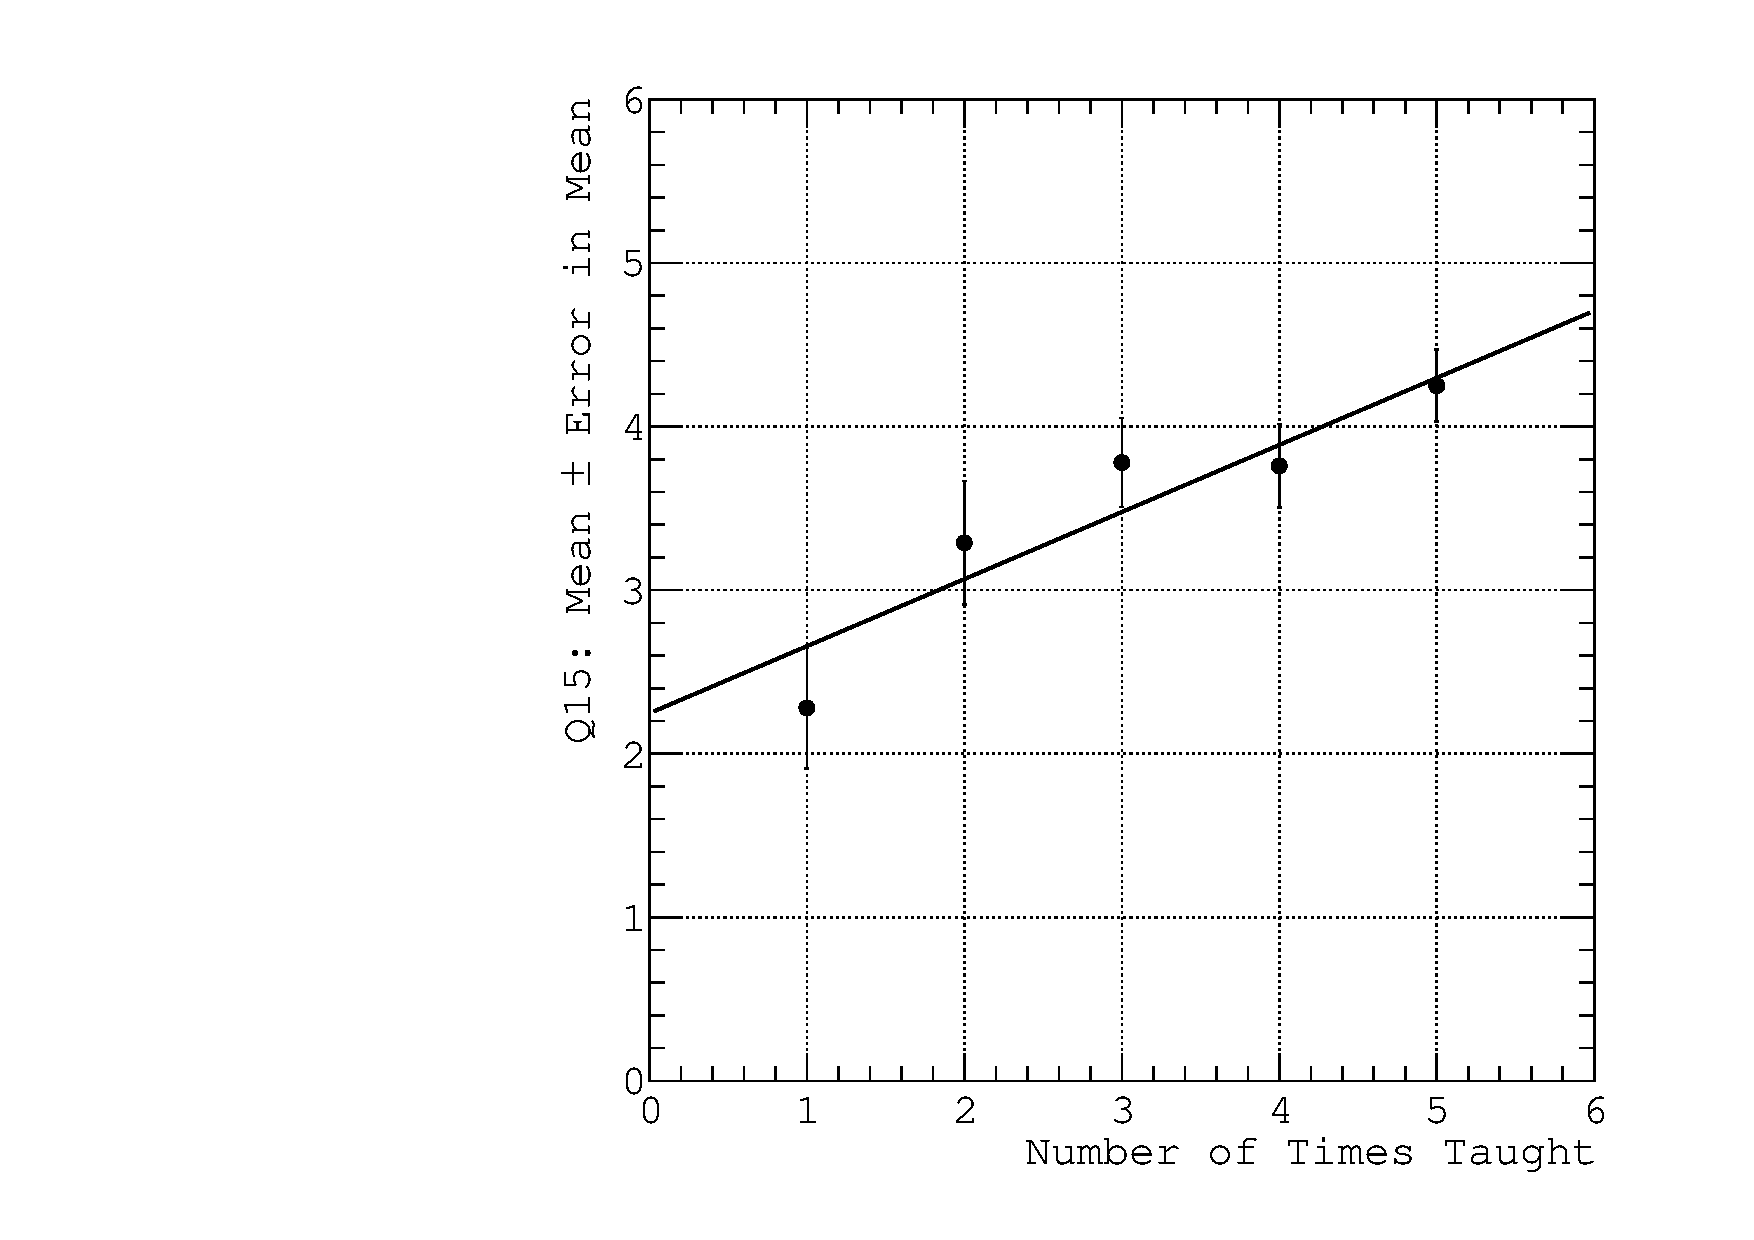
\includegraphics[width=0.4\textwidth]{Q15_algebra_based.pdf}
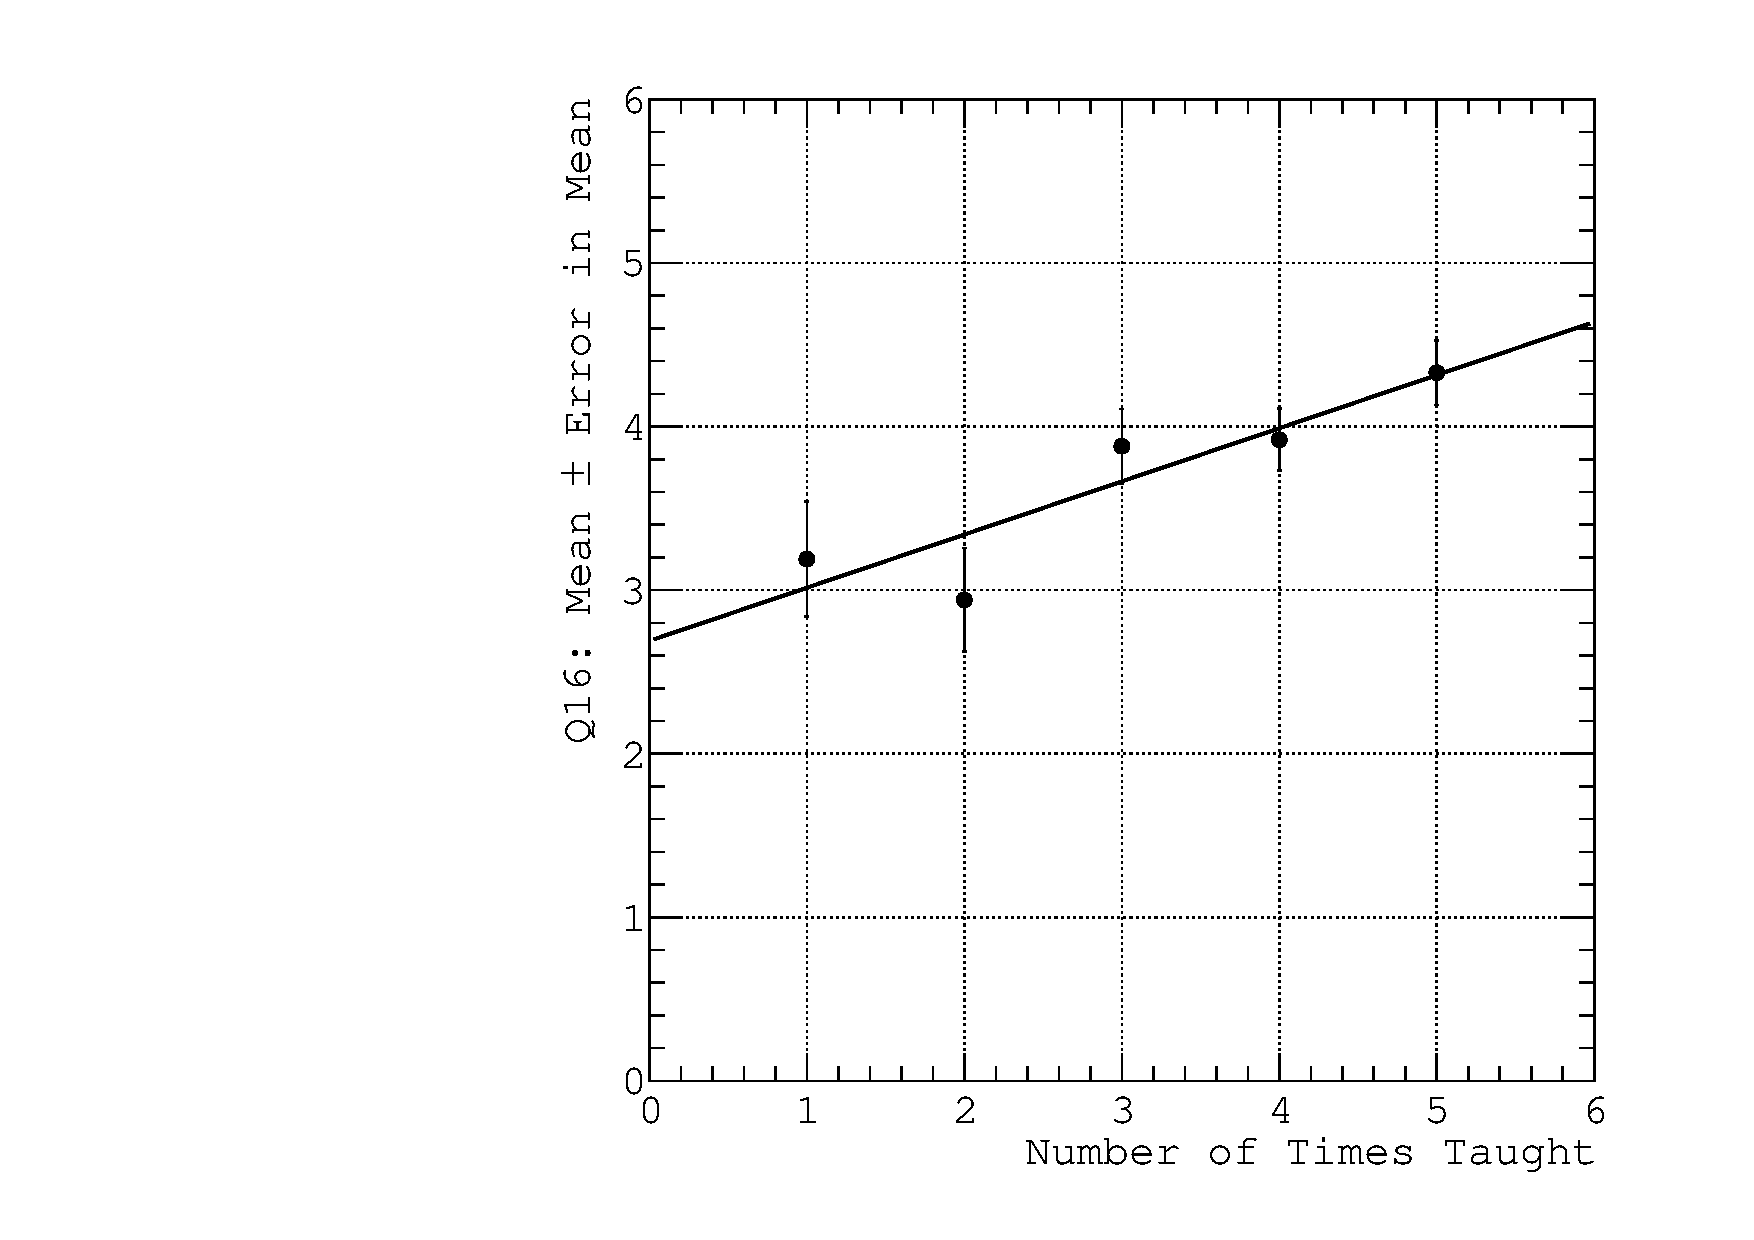
\includegraphics[width=0.4\textwidth]{Q16_algebra_based.pdf}
\caption{\label{fig:courses:intro_q15}  (Left) Student responses to Question 15 in algebra-based physics versus number of times taught. (Right) Student responses to Question 16 in algebra-based physics versus number of times taught.  The y-axis of the data points are the mean values, and the errors are the standard error in the mean.  The x-axis of the data points correspond to each time I've taught these courses.  The solid black lines are best-fit linear trend lines that minimize the $\chi^2$ value.}
\end{figure}

Approximately 40\% of PHYS135A/B students are kinesiology majors, and another 30\% are biology majors.  I have responded by creating modules focused on medical applications, and the article discussions also tie content from their chosen major to the course.  The results for questions 15-16 increase over time, as shown in Figure  \ref{fig:courses:intro_q15}.  \textbf{The mean values over time show an unmistakable and significant improvement}.  Further, the data in Tab. \ref{tab:courses:intro_shifts_1} show that \textit{every student evaluation measurement has increased}, with the exception of the question pertaining to course difficulty, Question 11\footnote{``This course was academically challenging.''}.  This was by design and in alignment with recommendations to slow the pace. \\ \hspace{0.1cm}

\begin{table}
\small
\centering
\begin{tabular}{| c | c | c | c | c |}
\hline
\hline
Question & First Time & Most Recent Time & Raw change & Standard deviations \\
\hline
10 & 3.76 $\pm$ 0.227 & 4.46 $\pm$ 0.159 & 0.7 $\pm$ 0.277 & 2.53 \\ \hline
11 & 4.57 $\pm$ 0.164 & 4.42 $\pm$ 0.159 & -0.15 $\pm$ 0.228 & -0.657 \\ \hline
12 & 4.29 $\pm$ 0.22 & 4.54 $\pm$ 0.159 & 0.25 $\pm$ 0.272 & 0.919 \\ \hline
13 & 3.52 $\pm$ 0.29 & 4.42 $\pm$ 0.19 & 0.9 $\pm$ 0.347 & 2.6 \\ \hline
14 & 3.48 $\pm$ 0.297 & 4.46 $\pm$ 0.169 & 0.98 $\pm$ 0.342 & 2.87 \\ \hline
15 & 3.29 $\pm$ 0.367 & 4.25 $\pm$ 0.21 & 0.96 $\pm$ 0.423 & 2.27 \\ \hline
16 & 3.19 $\pm$ 0.343 & 4.33 $\pm$ 0.188 & 1.14 $\pm$ 0.391 & 2.92 \\ \hline
17 & 4.24 $\pm$ 0.227 & 4.57 $\pm$ 0.149 & 0.33 $\pm$ 0.271 & 1.22 \\ \hline
18 & 3.52 $\pm$ 0.29 & 4.48 $\pm$ 0.174 & 0.96 $\pm$ 0.338 & 2.84 \\ \hline
19 & 3.48 $\pm$ 0.306 & 4.38 $\pm$ 0.167 & 0.9 $\pm$ 0.348 & 2.58 \\ \hline
20 & 4.24 $\pm$ 0.238 & 4.52 $\pm$ 0.174 & 0.28 $\pm$ 0.294 & 0.951 \\ \hline
21 & 4.48 $\pm$ 0.225 & 4.54 $\pm$ 0.169 & 0.06 $\pm$ 0.281 & 0.213 \\ \hline
22 & 4.1 $\pm$ 0.194 & 4.48 $\pm$ 0.202 & 0.38 $\pm$ 0.28 & 1.36 \\ \hline
23 & 3.95 $\pm$ 0.262 & 4.64 $\pm$ 0.135 & 0.69 $\pm$ 0.294 & 2.34 \\ \hline
24 & 4.67 $\pm$ 0.127 & 4.75 $\pm$ 0.108 & 0.08 $\pm$ 0.167 & 0.48 \\ \hline
25 & 3.24 $\pm$ 0.338 & 4.46 $\pm$ 0.169 & 1.22 $\pm$ 0.378 & 3.22 \\ \hline
\hline
\end{tabular}
\caption{\label{tab:courses:intro_shifts_1} Comparison algebra-based numbers for the first time taught (first column) to the most recent time (second column). The raw change is given in the third column, and the change divided by the standard deviation is given in the fourth column.}
\end{table}

In following FPC and department recommendations, I have made three modifications to 135A/B.  First, the pace has been decreased.  Second, I have included more step-by-step exampled.  Third, I have included more traditional lecture content.  Although there is a decrease in course difficulty, the most recent value for question 11 was still $4.46 \pm 0.159$.  When I put these changes in place, some students expressed such relief that they told me in office hours.  One student joked that ``You could be an online professor for Chegg.com!'' He was complimenting my style by referencing an online resource where instructors demonstrate solutions to physics problems in step-by-step traditional style.  \\ \hspace{0.1cm}

Struggling students copy examples verbatim, comparing new problems to these examples for reference.  I've learned recently that more structure is especially helpful when trying to create more \textbf{inclusive classrooms} \cite{inclusive}. Figure \ref{fig:courses:intro_q15} demonstrates measurable improvement for the first introductory course learning focus (curiosity) by \textit{measurably increasing the interest of the students in physics} (Fig. \ref{fig:courses:intro_q15}).  The simple classroom pattern of 1) traditional content introducing concept 2) slow step-by-step example 3) PI module 4) laboratory activity/PhET seems to increase student engagement and interest in the material.  Examples of student-designed experiments and presentations are included in the Supplemental Material, which also serve the first learning goal.\\ \hspace{0.1cm}

Another improvement strategy came from ch. 4 of Eric Mazur's work on PI modules \cite{mazur}.  I now write the simplified class agenda shortly before class time.  I ensure that it contains no more than 4-5 items, and I present it to the students.  This benefits the students in two ways.  First, basing the agenda on the students' progress to-date helps me to find the correct course pace.  Second, keeping the agenda simple and explaining it to the class communicates further structure to the students, priming them for the next 90 to 120 minutes.  As part of the agenda, I provide a list of equations used that day in the \textit{memory bank}.  Third, I remind the students of current homework and specific chapter sections I expect them to do in the next few days.  In 2018, a student suggested I break the reading into small sections.  This prompts the students to focus on the 10-20 pages relevant for that day.  An example agenda is shown in Fig. \ref{fig:courses:intro:exampleAgenda} in Sec. \ref{sec:courseDesc}. \\ \hspace{0.1cm}

Two additional comments are relevant regarding the introductory course pace.  First, the number of textbook chapters covered in PHYS135A/B was not reduced.  By attending the classes taught by Profs. Zorba and Lagan, I obtained a better sense of \textit{how much} content within each chapter is covered.  Drs. Zorba and Lagan have been very helpful in demonstrating how to best set the course pace.  Professor Piner has also attended lectures in my recent classes and offered useful and positive feedback.  Second, we removed the topics of physical oscillations from PHYS150, and thermodynamics and optics from PHYS180.  In the past, PHYS180 was a 5.0 credit course.  In 2018-2019 we decided to create a calculus-based physics III called PHYS185 which now contains the thermodynamics, oscillations, and optics topics.  The number of chapters for PHYS180 is now reduced by 30\%.  Through these actions, my department and I are working together to accommodate our students.  \\ \hspace{0.1cm}

\begin{figure}[h]
\centering
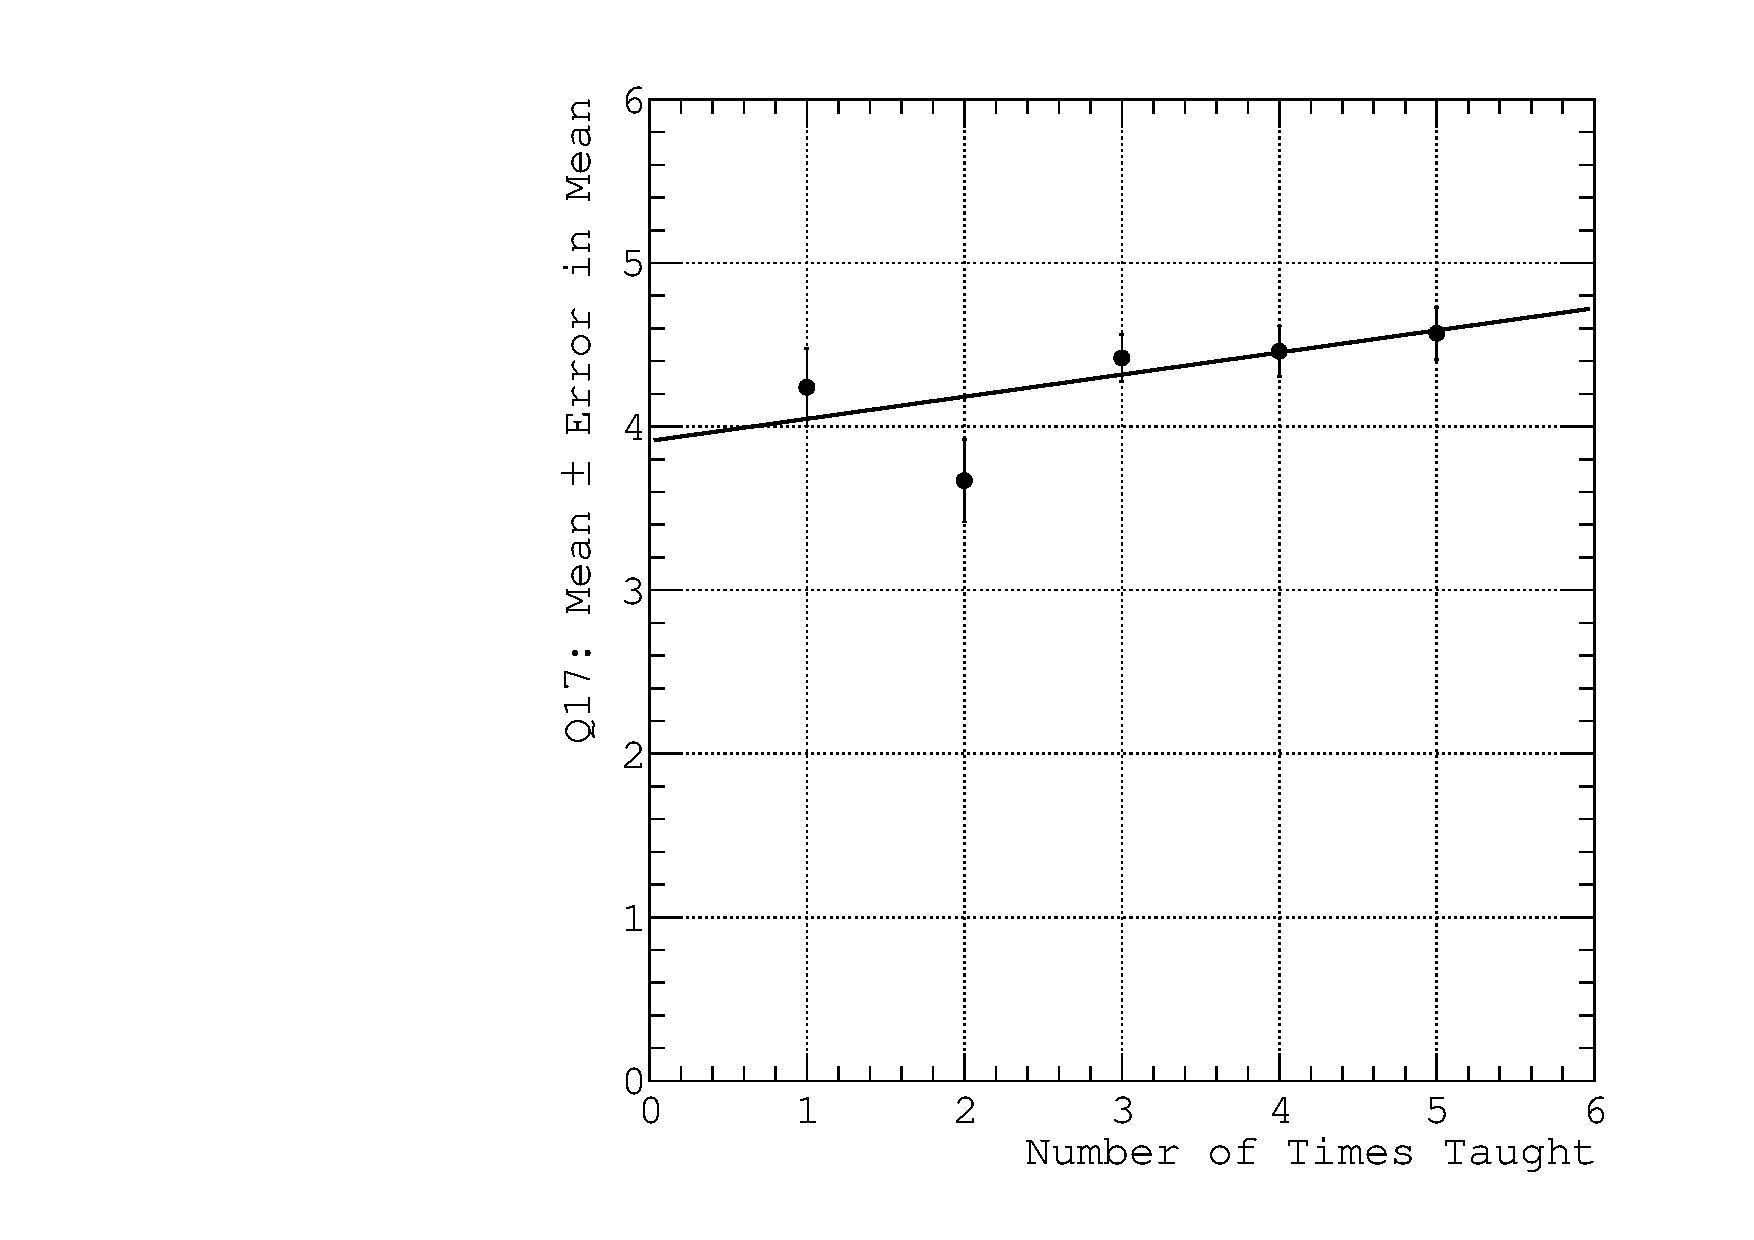
\includegraphics[width=0.4\textwidth]{Q17_algebra_based.pdf}
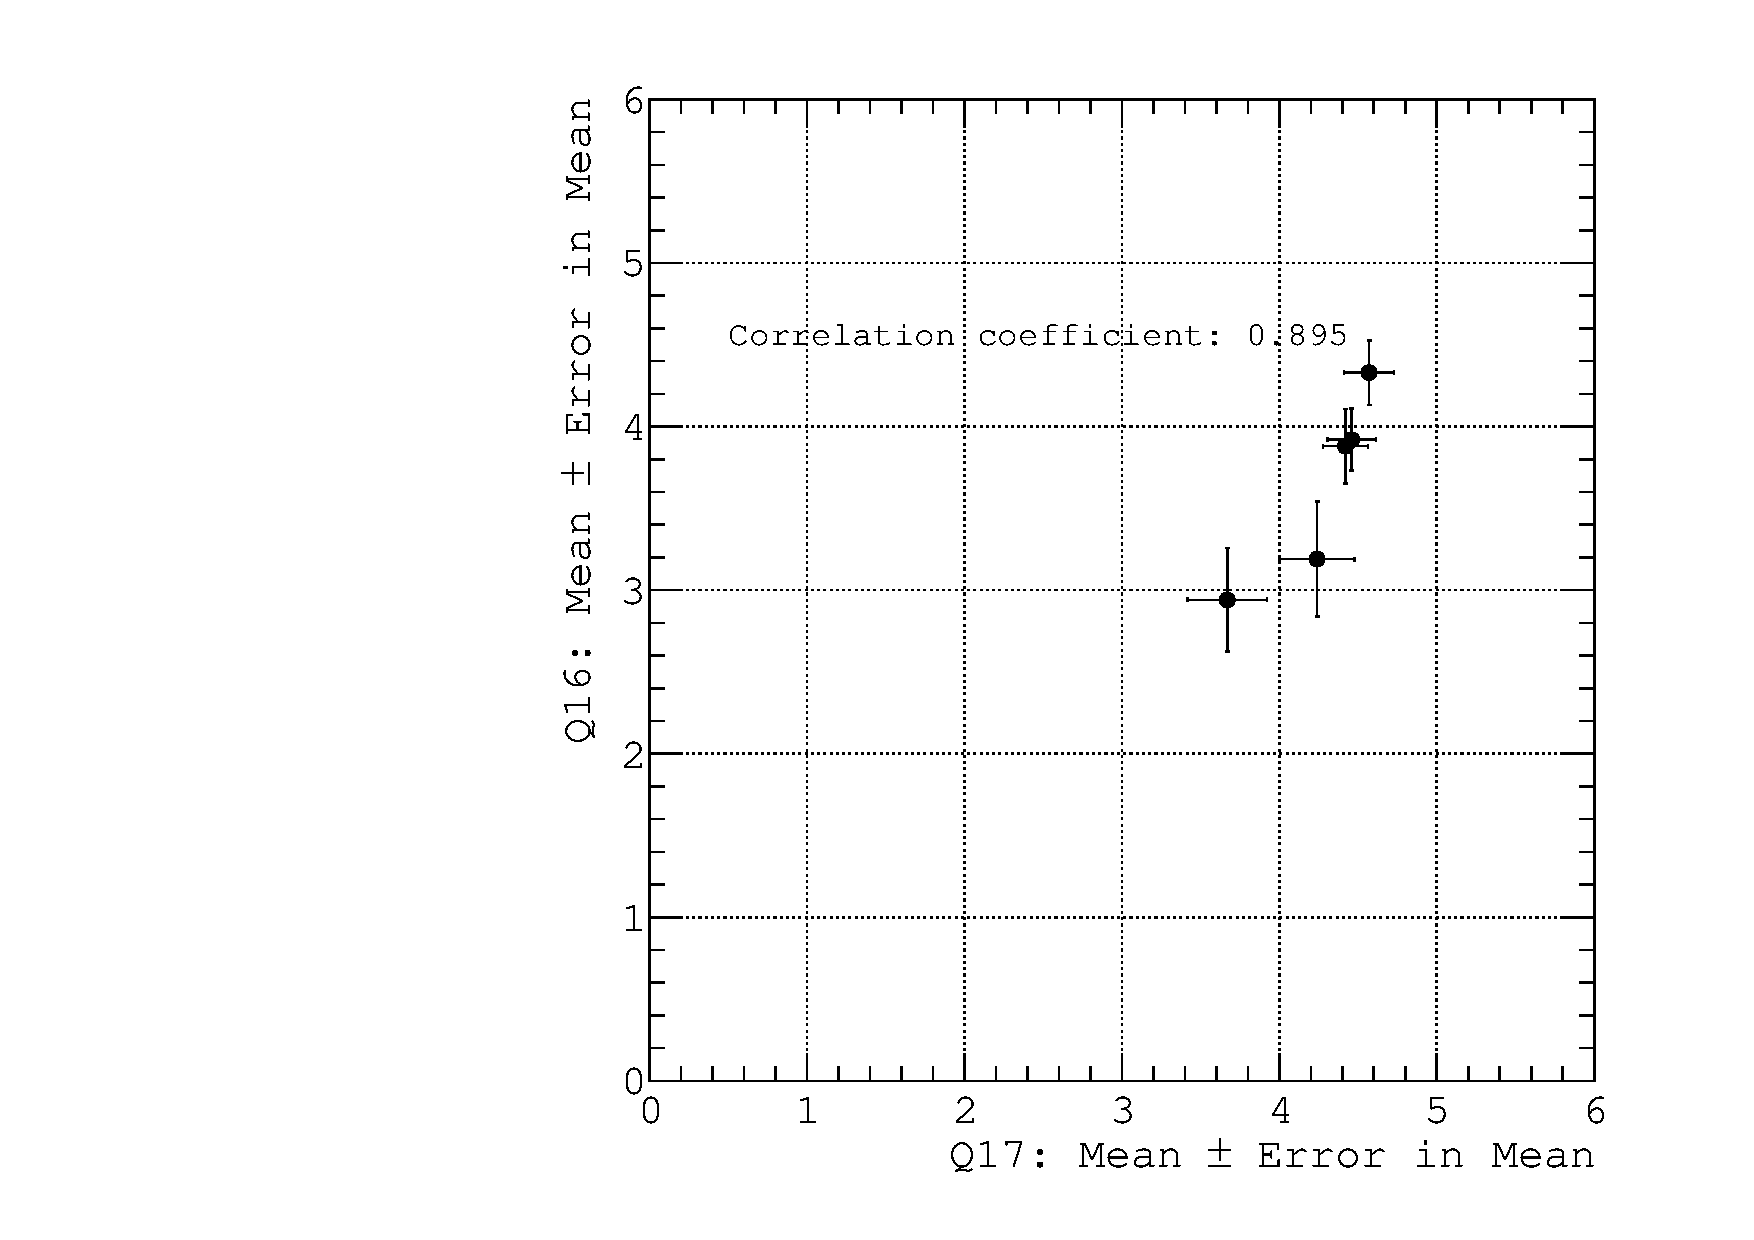
\includegraphics[width=0.4\textwidth]{Q16_Q17_algebra_based.pdf}
\caption{\label{fig:courses:intro_q17}  (Left) Student responses (mean values and errors in the mean) to Question 17 in algebra-based physics versus number of times taught. (Right) Student responses to Question 16 in algebra-based physics versus responses to Question 17.  The x and y-axis values of the data points are the mean values, and the errors are the errors in the mean.}
\end{figure}

My department also recommended that I focus on question 17\footnote{``The professor used class time effectively and demonstrated preparation for class''.}.  Question 17 results are shown in Fig. \ref{fig:courses:intro_q17}.  My department suggested question 17 is correlated with other key measurements like question 16.  Figure \ref{fig:courses:intro_q17} (right) shows that the Pearson correlation coefficient is 0.895.  Anecdotally, the JITT modules probably contributed to lower question 17 mean values in Spring 2018 (x-value of 2 in Fig. \ref{fig:courses:intro_q17}, left).  These modules involve analyzing student responses to questions assigned one day before class and modifying course content based on their responses.  The idea is to tailor course content, however, it was common for struggling students to not respond rather than risk submitting wrong answers.  I reassured them that the response data was useful and that they were being graded for completion, not accuracy, but the response rates hovered around 50-60\%.  It became difficult therefore to modify the upcoming content as prescribed by JITT.  I have subsequently dropped JITT modules.  \\ \hspace{0.1cm}

\begin{figure}
\centering
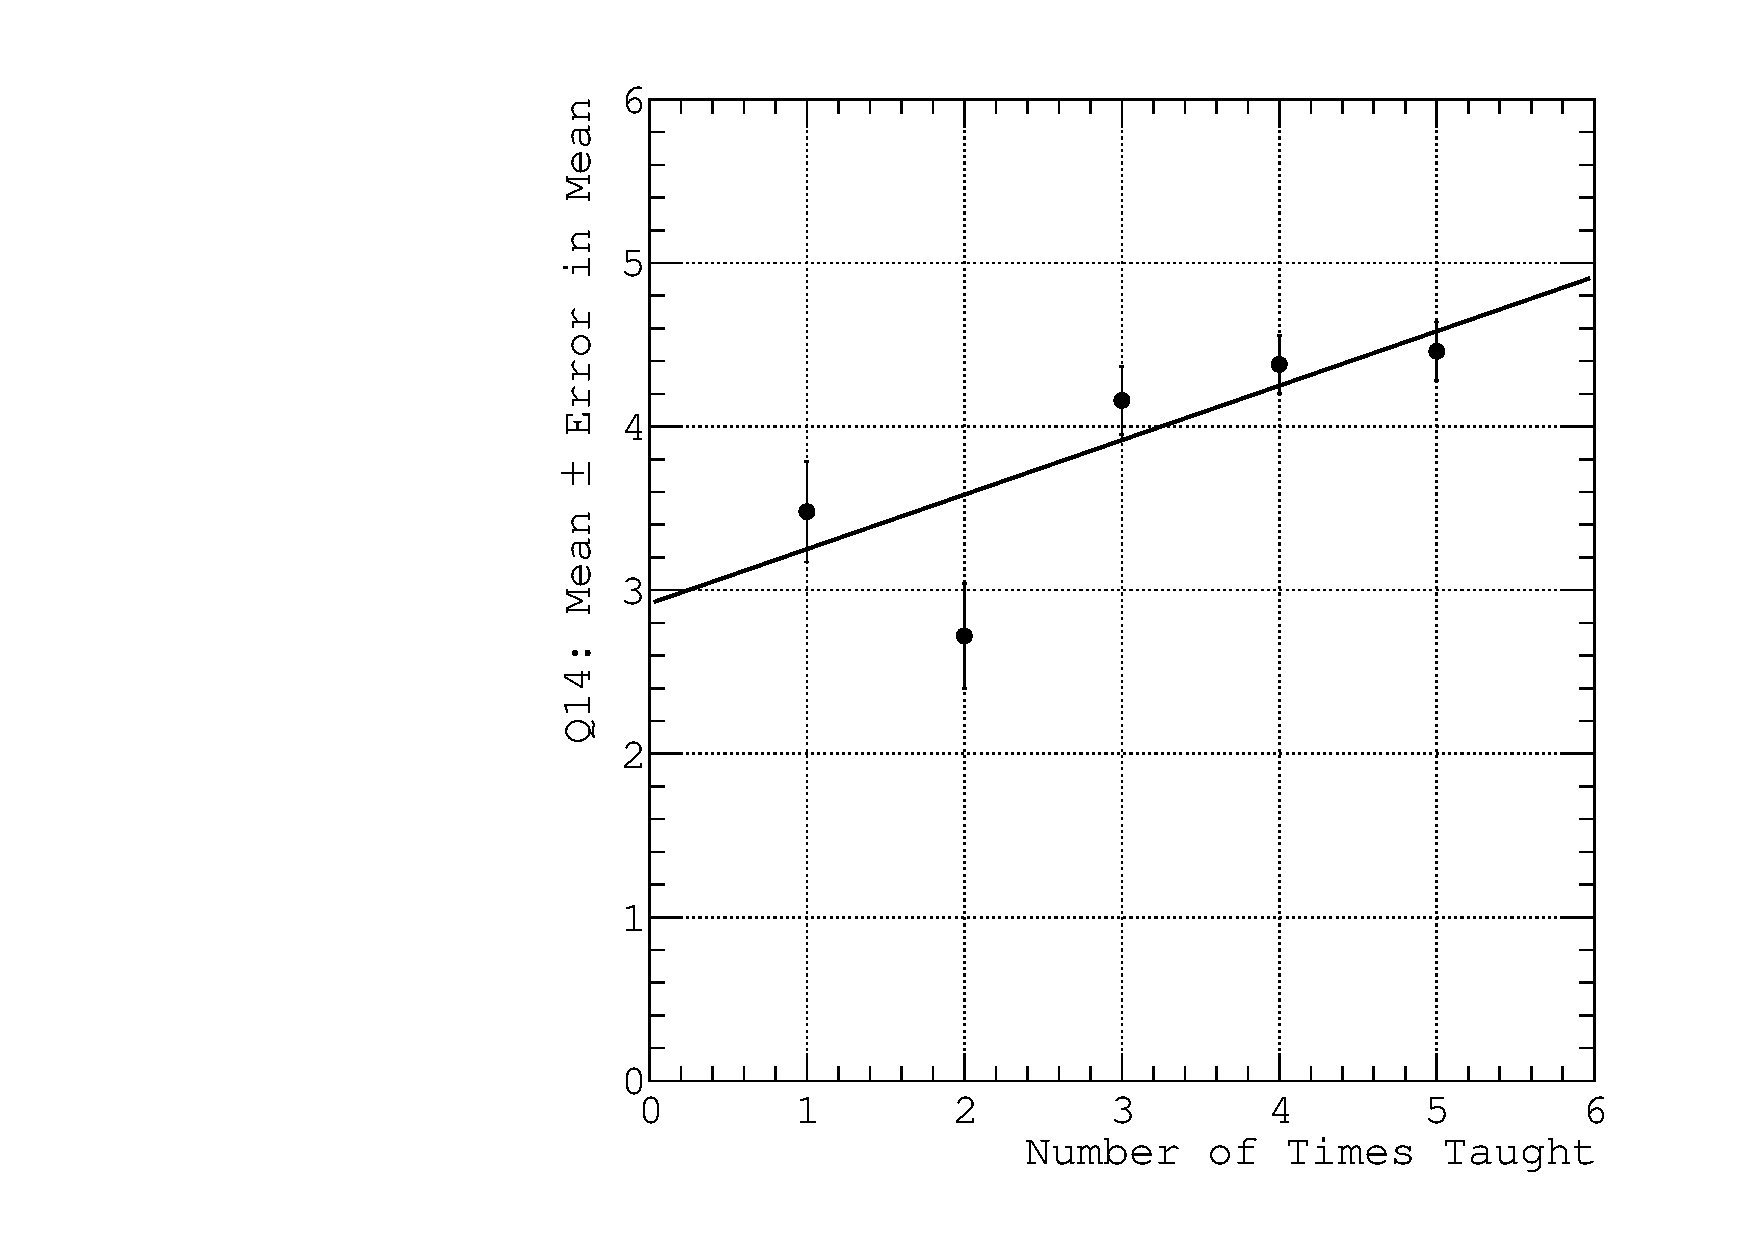
\includegraphics[width=0.4\textwidth]{Q14_algebra_based.pdf}
\caption{\label{fig:courses:intro_q14}  Student responses (mean values and errors in the mean) to Question 14 in algebra-based physics versus number of times taught.  The solid black lines are best-fit linear trend lines that minimize the $\chi^2$ value.}
\end{figure}

The second of my three learning focuses for introductory physics courses is to improve the analysis skill of the students.  My strategy of combined traditional and PER based content appears to be working as I improve it over time.  Figure \ref{fig:courses:intro_q14} contains student response data to Question 14\footnote{``This course  improved my understanding of the material.''}.  The data point well-below the trend line corresponds to the PHYS135B section in which I introduced JITT modules.  Since then I have removed that type of module and implemented the three main changes (control of the pace, step-by-step examples, and more traditional content).  \textbf{The student response data shows that their understanding of the material is improving substantially.}  The linear trend suggests that with each subsequent round of teaching algebra-based physics, the modified approach we are taking in these courses will continue to yield good results for our students in this area.  \\ \hspace{0.1cm}

\begin{figure}
\centering
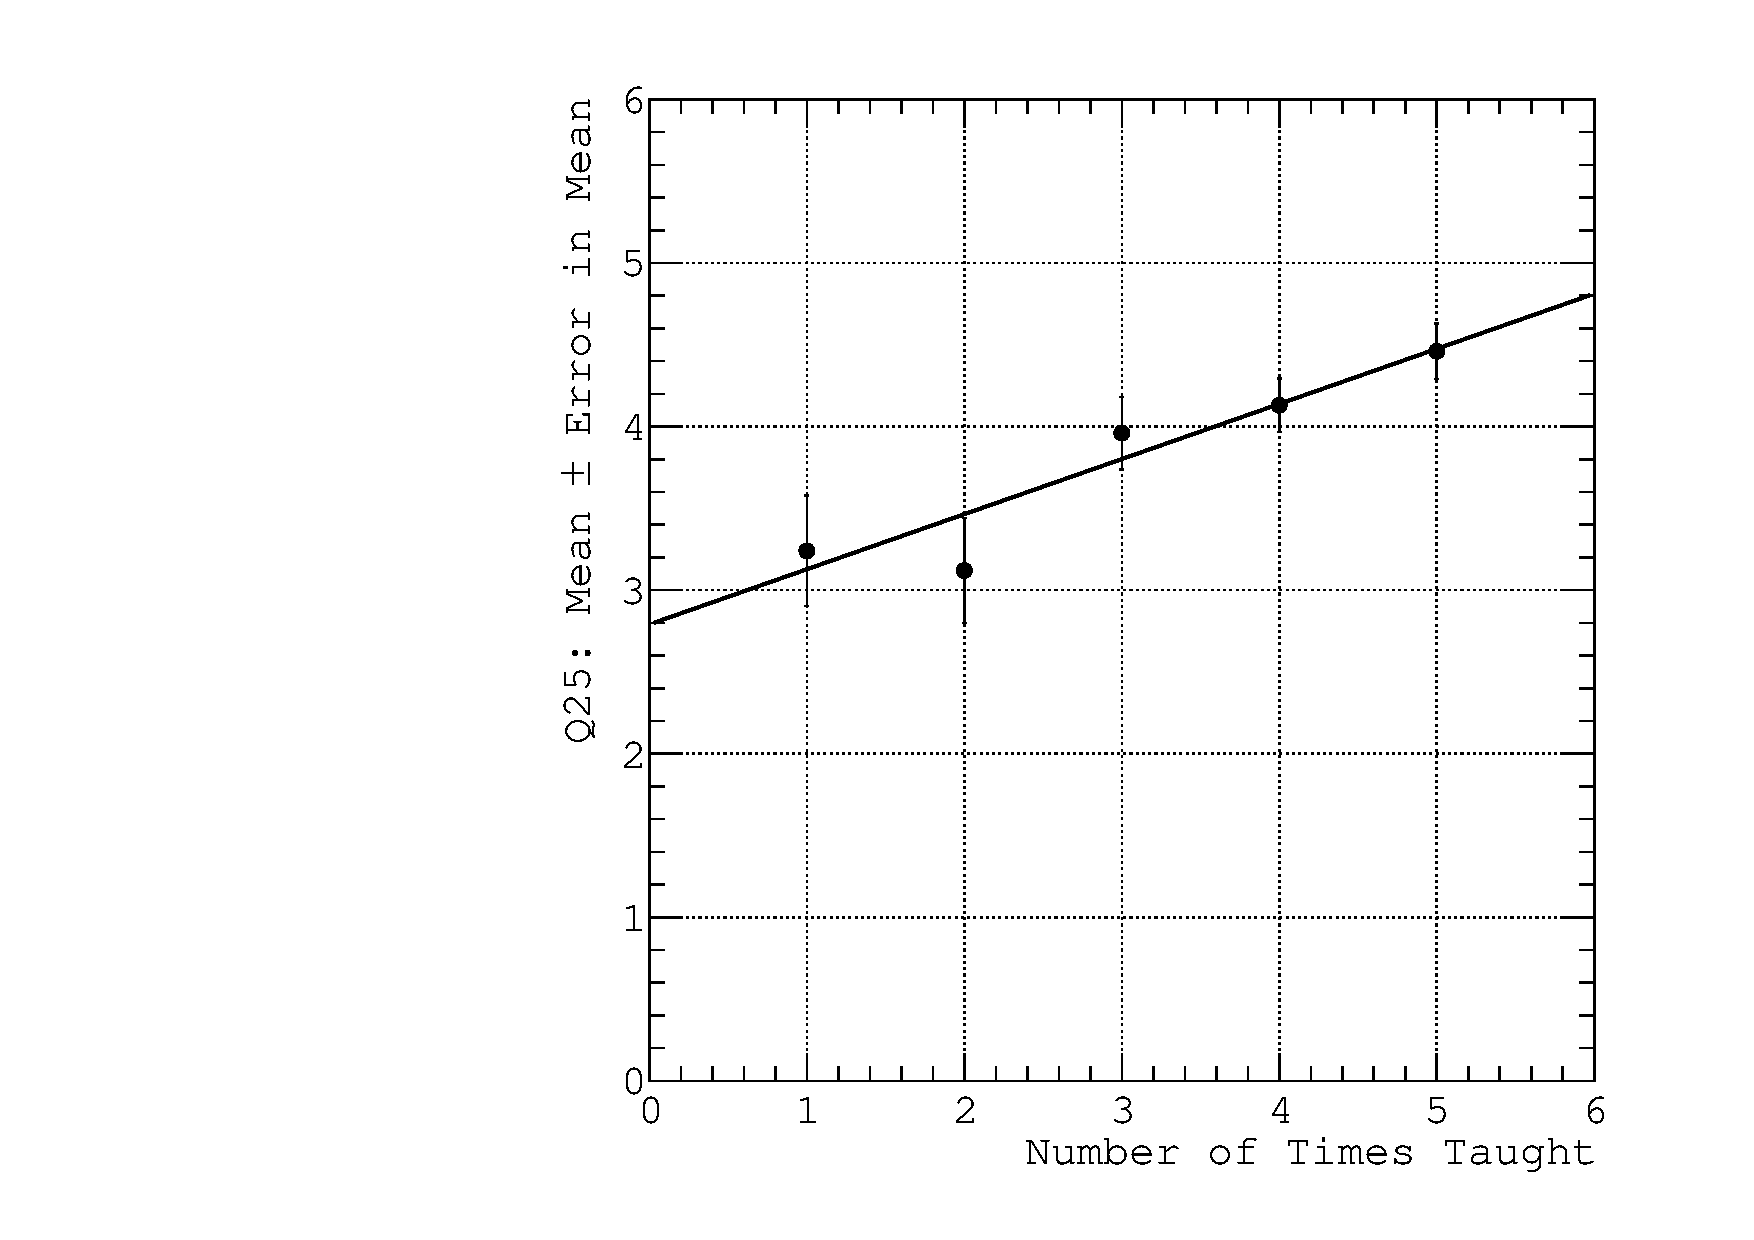
\includegraphics[width=0.4\textwidth]{Q25_algebra_based.pdf}
\caption{\label{fig:courses:intro_q25}  Student responses (mean values and errors in the mean) to Question 25 in algebra-based physics versus number of times taught.  The solid black lines are best-fit linear trend lines that minimize the $\chi^2$ value.}
\end{figure}

The third of my learning focuses is \textit{applications to society}, with measurable goals of requiring the students to present articles they find relevant due to societal impact and to manage and aid in student-designed experiments presented in class.  I have included examples of my students' wonderful work in this area in the Supplemental Material, including both articles and student-designed experiments.  For the experiments and presentations of the results, groups have correctly predicted maximum model rocket flight times, measured the speed of sound with musical intruments, and build DC circuits from citrus fruits.  The articles the students chose were often thought-provoking, and related to their field of interest, including medicine and environmental science.  My questions during their discussions would usually steer them back to the physics involved, and the class would therefore learn about the utility of physics in situations beyond the classroom.  I have included example articles we covered in the Supplemental Materials.  Perhaps my favorite was an inspiring case study in which a University of Texas undergraduate used machine learning to help find extra-solar planets.

Finally, I am thrilled to report an increase in student responses to Question 25\footnote{``Overall, I would recommend this professor to others.''}. \textbf{Figure \ref{fig:courses:intro_q25} contains Question 25 mean values over time, and the data show an unmistakable and significant improvement.}  It turns out there has been similar improvement in the calculus-based versions of the introductory physics courses I teach.  By thoughtfully implementing the changes recommended to me by my department and FPC, I see in the data that the students are endorsing me as their professor at increasing mean values over time.  I have found upon reflecting on algebra-based physics methods, that the final piece of the puzzle was to \textit{build relationships} with the students.  What follows are anecdotal stories from class that illustrate what I was able to accomplish by building relationships with students who needed help with a difficult subject.  \\ \hspace{0.1cm}

\subsection{Anecdotes from Class, Relationships with Introductory Physics Students}

My first story involves a senior Kinesiology major named LaJana Morris.  LaJana found the courage to approach me during the test, and ask a question about a problem.  The exercise required the students to write an equation based on the words, and solve for the missing variable $x$.  It appeared that LaJana was close to forming the correct equation, and I asked her to think conceptually about which equation from her equation sheet she should be trying to deploy.  Eventually she chose the correct one, based on the context.  I assumed she'd be able to finish, given that the problem was now reduced to solving for $x$.  I will never forget her next words: ``How do I move $x$ to get it by itself, without plugging in numbers?''  I was shocked and disappointed as I began to realize LaJana was \textit{unfamiliar with the concept of algebra.}  Of course I did not blame the student, but the question in my mind was: ``Who allowed this to happen?''  Knowing that this was a college senior who had never been shown algebra, I knuckled down and resolved to get the job done.  I made it my personal mission to ensure that LaJana passed my class, and she did.  Her midterm grades improved, and by the end of the course we were both pleased.  \\ \hspace{0.1cm}

My second story involves a senior WSP major named Jasmine Cao who was my student in PHYS135A/B.  Jasmine is an example of an excellent student who intends to apply to medical school.  Three main changes I put in place for the algebra-based physics were to slow and control the pace, include more examples, and include more traditional lecture content.  As part of the pace control I would include more group discussion time in PI modules, and I would focus my attention on tables of students I knew were struggling.  Jasmine and her friends formed a table that almost never struggled.  I worried that my new tactics would leave students like these feeling ignored.  However, by the end of the course, Jasmine told me they had a wonderful experience!  Apparently I was able to balance my focus enough such that no one student felt left out.  Jasmine's Thank You note is included in the Supplemental Material.  \\ \hspace{0.1cm}

My third story involves a senior Biology major named Daniel Diaz.  I identified Daniel as someone struggling with the material during my PI discussion rounds during PHYS135A and PHYS135B (2018-2019).  During our PI discussion rounds, I got the sense that Daniel was close to get the right answers but was just short of making the vital connections necessary for word-problem solving.  I made a concerted effort to spend more time at his table, and worked quick examples for their table during discussion time.  Not only did it benefit him but it benefit the three other students because I later observed him teaching them!  After the final exam he wrote me this note: \\ \hspace{0.1cm}

\textit{Thank you for a fun year!  Physics is hard, but I definitely learned more than I thought I would.} - Daniel Diaz \\ \hspace{0.1cm}

\subsection{Analysis of Calculus-Based Introductory Physics Student Evaluations}

\begin{table}
\small
\centering
\begin{tabular}{| c | c | c |}
\hline \hline
Question & 180-02 $N$ & 180-02 result \\ \hline
10 & 8 & $5.00\pm 0.00$ \\ \hline
11 & 8 & $5.00\pm 0.00$ \\ \hline
12 & 8 & $5.00\pm 0.00$ \\ \hline
13 & 8 & $5.00\pm 0.00$ \\ \hline
14 & 8 & $5.00\pm 0.00$ \\ \hline
15 & 8 & $5.00\pm 0.00$ \\ \hline
16 & 8 & $5.00\pm 0.00$ \\ \hline
\hline
\end{tabular}
\quad
\begin{tabular}{| c | c | c |}
\hline \hline
Question & 180-02 $N$ & 180-02 result \\ \hline
17 & 8 & $5.00\pm 0.00$ \\ \hline
18 & 8 & $5.00\pm 0.00$ \\ \hline
19 & 8 & $5.00\pm 0.00$ \\ \hline
20 & 8 & $5.00\pm 0.00$ \\ \hline
21 & 8 & $5.00\pm 0.00$ \\ \hline
22 & 8 & $4.75\pm 0.25$ \\ \hline
23 & 8 & $5.00\pm 0.00$ \\ \hline
24 & 8 & $5.00\pm 0.00$ \\ \hline
25 & 8 & $5.00\pm 0.00$ \\ \hline
\hline
\end{tabular}
\caption{\label{tab:courses:intro_eval_3} (Left) Mean and error in the mean for questions 10-16 on the student evaluation form, for PHYS180-02, taught in Spring 2019.  These questions pertain to the \textit{course}.  (Right) Mean and error in the mean for questions 17-25 on the student evaluation form, for PHYS180-02, taught in Spring 2019.  These questions pertain to the \textit{professor}.}
\end{table}

\begin{table}
\small
\centering
\begin{tabular}{| c | c | c | c | c |}
\hline
\hline
Question & First Time & Most Recent Time & Raw change & Standard deviations \\
\hline
10 & 4.19 $\pm$ 0.207 & 5 $\pm$ 0 & 0.81 $\pm$ 0.207 & 3.9 \\ \hline
11 & 4.19 $\pm$ 0.345 & 5 $\pm$ 0 & 0.81 $\pm$ 0.345 & 2.35 \\ \hline
12 & 3.63 $\pm$ 0.327 & 5 $\pm$ 0 & 1.37 $\pm$ 0.327 & 4.18 \\ \hline
13 & 4 $\pm$ 0.275 & 5 $\pm$ 0 & 1 $\pm$ 0.275 & 3.64 \\ \hline
14 & 3.93 $\pm$ 0.333 & 5 $\pm$ 0 & 1.07 $\pm$ 0.333 & 3.22 \\ \hline
15 & 3.56 $\pm$ 0.315 & 5 $\pm$ 0 & 1.44 $\pm$ 0.315 & 4.57 \\ \hline
16 & 3.56 $\pm$ 0.315 & 5 $\pm$ 0 & 1.44 $\pm$ 0.315 & 4.57 \\ \hline
17 & 3.31 $\pm$ 0.285 & 5 $\pm$ 0 & 1.69 $\pm$ 0.285 & 5.93 \\ \hline
18 & 2.88 $\pm$ 0.34 & 5 $\pm$ 0 & 2.12 $\pm$ 0.34 & 6.24 \\ \hline
19 & 3.13 $\pm$ 0.385 & 5 $\pm$ 0 & 1.87 $\pm$ 0.385 & 4.86 \\ \hline
20 & 3.69 $\pm$ 0.312 & 5 $\pm$ 0 & 1.31 $\pm$ 0.312 & 4.19 \\ \hline
21 & 3.88 $\pm$ 0.273 & 5 $\pm$ 0 & 1.12 $\pm$ 0.273 & 4.11 \\ \hline
22 & 3.81 $\pm$ 0.333 & 4.75 $\pm$ 0.251 & 0.94 $\pm$ 0.417 & 2.26 \\ \hline
23 & 3.67 $\pm$ 0.343 & 5 $\pm$ 0 & 1.33 $\pm$ 0.343 & 3.88 \\ \hline
24 & 4.5 $\pm$ 0.157 & 5 $\pm$ 0 & 0.5 $\pm$ 0.157 & 3.17 \\ \hline
25 & 3.13 $\pm$ 0.407 & 5 $\pm$ 0 & 1.87 $\pm$ 0.407 & 4.59 \\ \hline
\hline
\end{tabular}
\caption{\label{tab:courses:intro_shifts_2} Comparison calculus-based numbers for the first time taught (first column) to the most recent time (second column). The raw change is given in the third column, and the change divided by the standard deviation is given in the fourth column.}
\end{table}

As with the algebra-based courses, the data from the 2018-2019 academic year for the \textit{calculus-based} courses demonstrates significant improvement in my teaching methods.  Table \ref{tab:courses:intro_eval_3} contains student evaluation data from PHYS180 for 2019.  In Tab. \ref{tab:courses:intro_shifts_2} the student evaluation data from the \textit{first} time I taught calculus-based physics is compared to the most \textit{recent} time.  The mean values and errors in the mean are shown from the responses to student evaluation questions 10-25 for both tables.  Questions 10-16 pertain to the course (Tab. \ref{tab:courses:intro_eval_3}, left), and questions 17-25 pertain to the professor (Tab. \ref{tab:courses:intro_eval_2}, right).  The data reflect high quality teaching and a substantial improvement compared to the first time I taught calculus-based physics. \\ \hspace{0.1cm}

The PHYS180 section from which the data in Tab. \ref{tab:courses:intro_eval_3} is derived shows almost perfect scores.  This is partly a credit to the changes I've put in place, and the reflecting I have done this past year.  However, it is also due to two other factors.  First, the aforementioned rearrangement of the thermodynamics curriculum made our lives easier in PHYS180.  Second, I had the chance to get acquainted with these students as advisees in the prior Fall 2018 semester before teaching them in Spring 2019.  Thus, reducing the pace of content and building relationships before class also made the course go much more smoothly. \\ \hspace{0.1cm}

The students in the PHYS180 course from 2019 were a combination of physics majors, 3-2 engineering program majors, and computer science.  I knew this particular set of students from Fall 2018, when I shadowed Dr. Lagan as he mentored them during Freshman Orientation.  By forming a relationship with them early on, I think they trusted that the class activities and methods I chose for them were for the best.  I performed my three usual changes to the course style (slower pace, more examples, and traditional content).  I followed with PI modules and laboratory activities/PhET activities.  They dived in to the PI modules with fervor, and we had many interesting discussions. \\ \hspace{0.1cm}

Something that made the PI module process different than algebra-based physics was that there were only two students per table.  Thus, each time I addressed a table when they hadn't gotten the answer yet, I was speaking with half the usual number of students compared to algebra-based physics.  This seemed to reduce complications and make my life easier.  When speaking with the usual four students in algebra-based physics, I sometimes notice that I can turn the light on in three students and one will stay quiet.  Although I try to reach everyone, it is sometimes awkward when I have other tables to approach and a limited time.  The smaller class-size of PHYS180 (2019) didn't have this problem and I was able to target struggling students with speed and accuracy.  There were originally nine students in my section of PHYS180, but one dropped the course because he was struggling to balance varsity sports and studying.  I welcomed him to office hours to discuss his priorities, but ultimately he had to rearrange his schedule and postpone PHYS180. \\ \hspace{0.1cm}

\begin{figure}
\centering
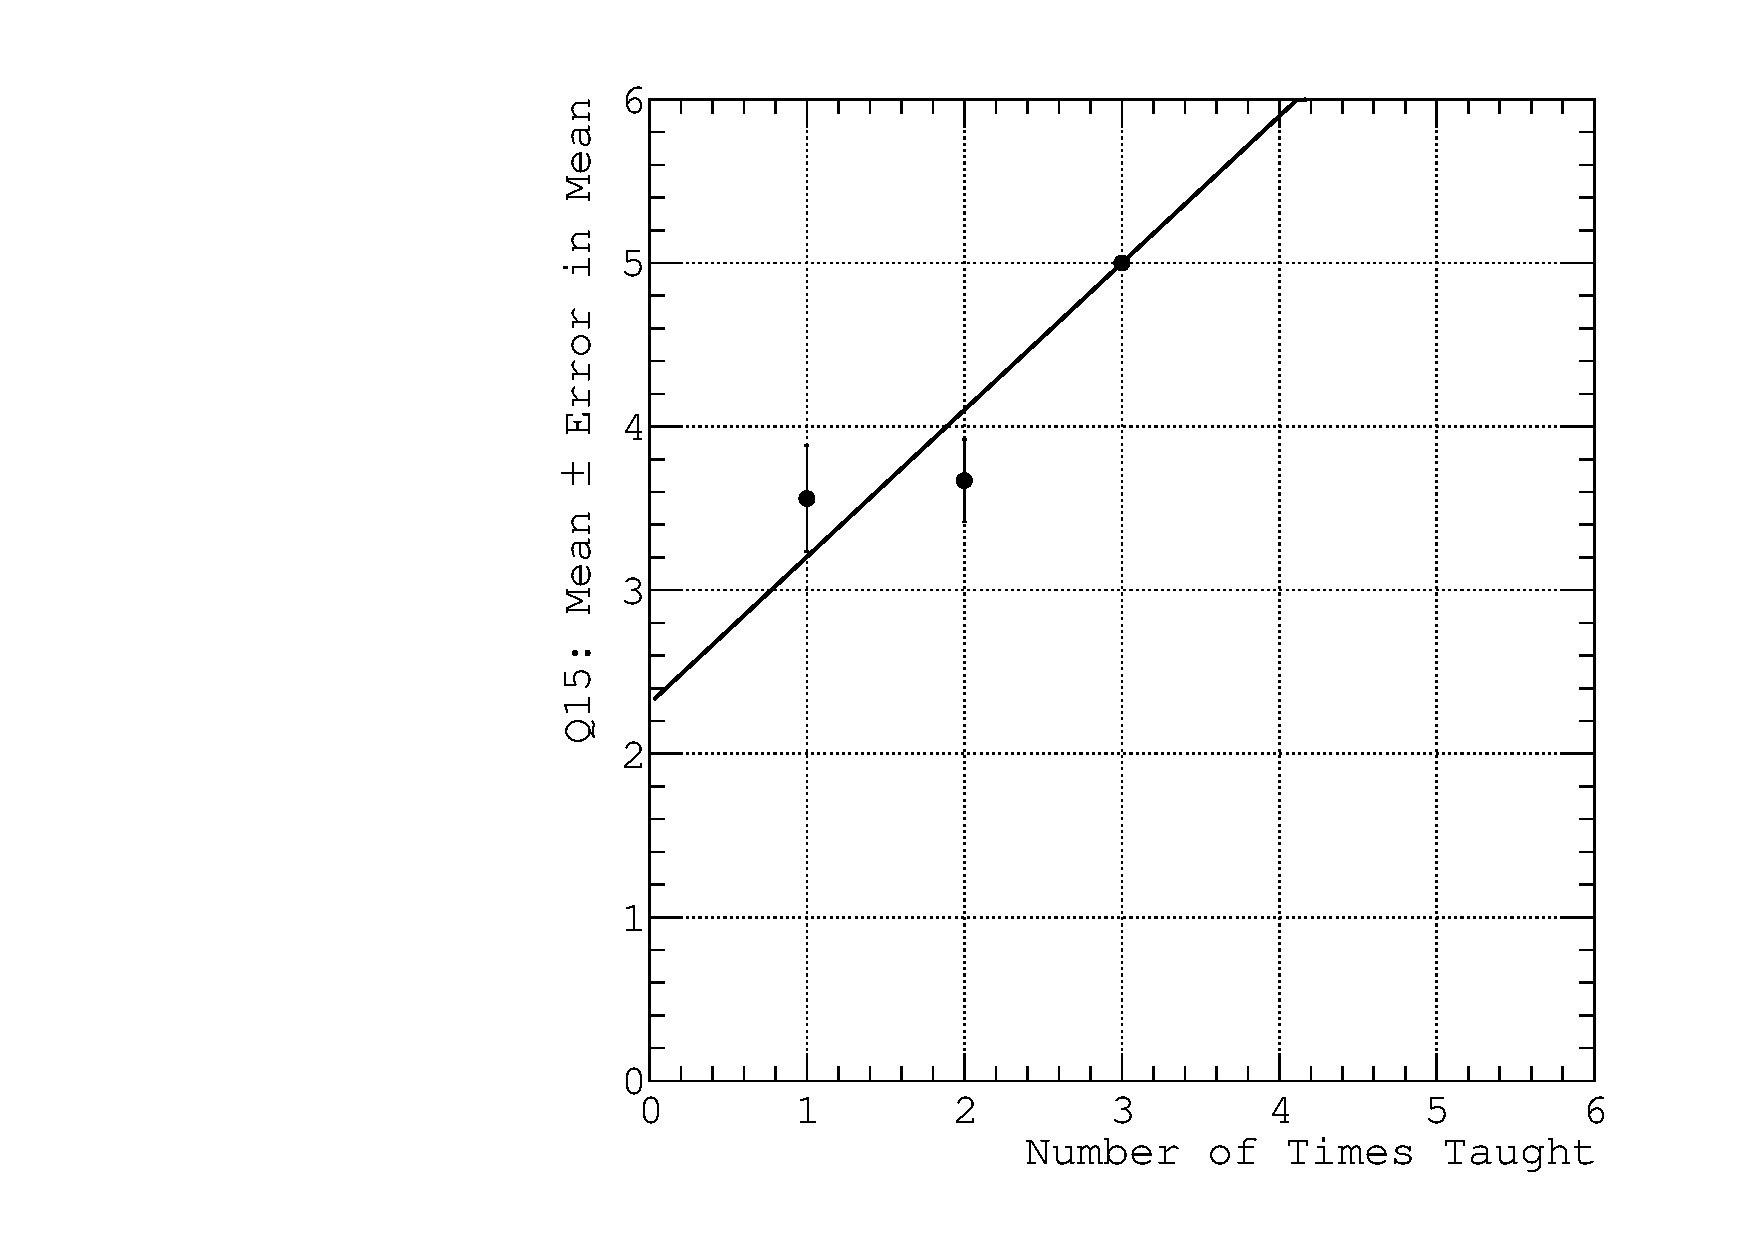
\includegraphics[width=0.4\textwidth]{Q15_calculus_based.pdf}
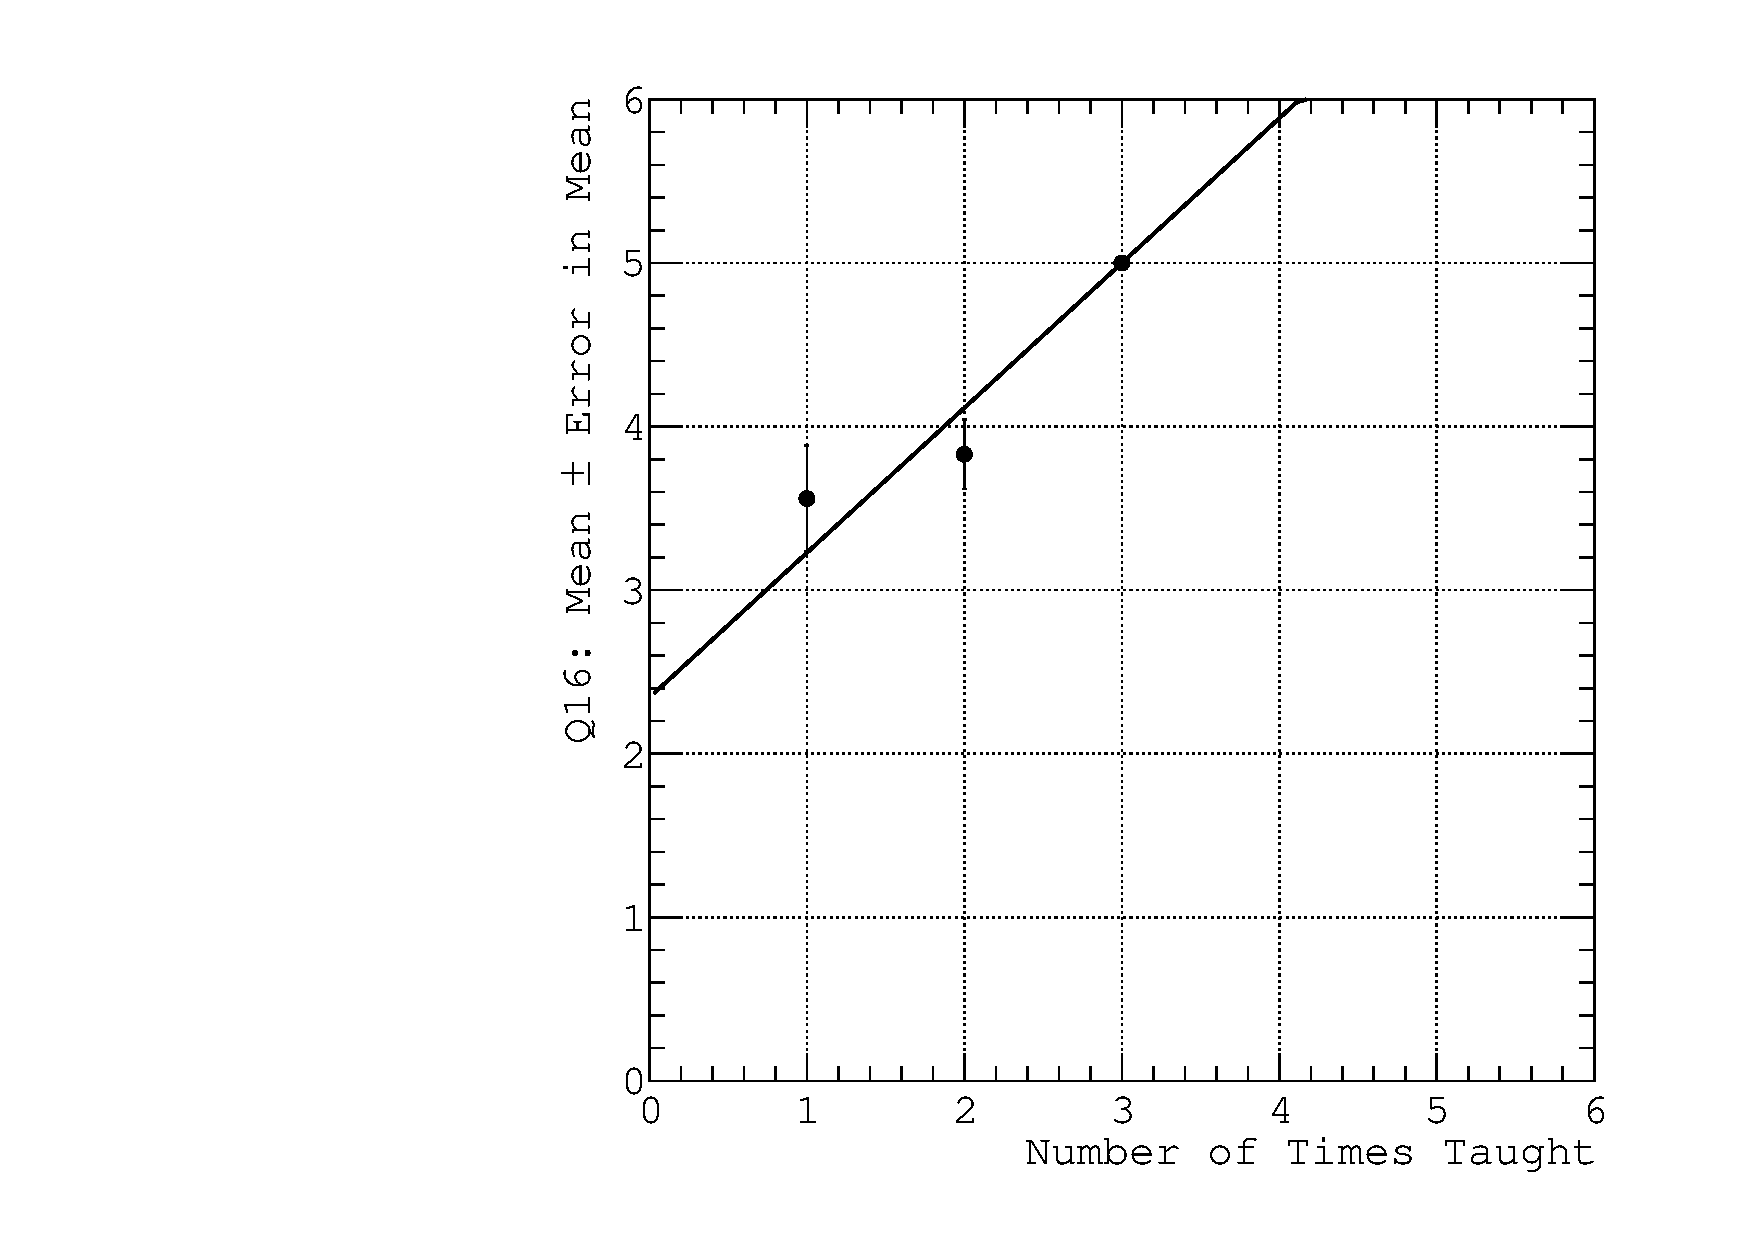
\includegraphics[width=0.4\textwidth]{Q16_calculus_based.pdf}
\caption{\label{fig:courses:intro_q15_2}  (Left) Student responses to Question 15 in calculus-based physics versus number of times taught. (Right) Student responses to Question 16 in calculus-based physics versus number of times taught.  The y-axis of the data points are the mean values, and the errors are the standard error in the mean.  The x-axis of the data points correspond to each time I've taught these courses.  The solid black lines are best-fit linear trend lines that minimize the $\chi^2$ value.}
\end{figure}

Figure \ref{fig:courses:intro_q15_2} shows the evolution of student responses to Questions 15-16 over time\footnote{Question 15: ``This course increased my interest in the subject matter,'' Question 16: ``Overall, I would recommend this course to others.''}.  The data show that I am perfecting my ability to boost student curiosity over time, in satisfaction of my first learning focus for introductory courses.  The final data point drives the trend line since it has no error.  Needless to say I look forward to teaching PHYS150 this Fall 2019 with my new advisees.  This upcoming semester will be the first time I've been a freshman mentor and adviser to my own students.

\begin{figure}
\centering
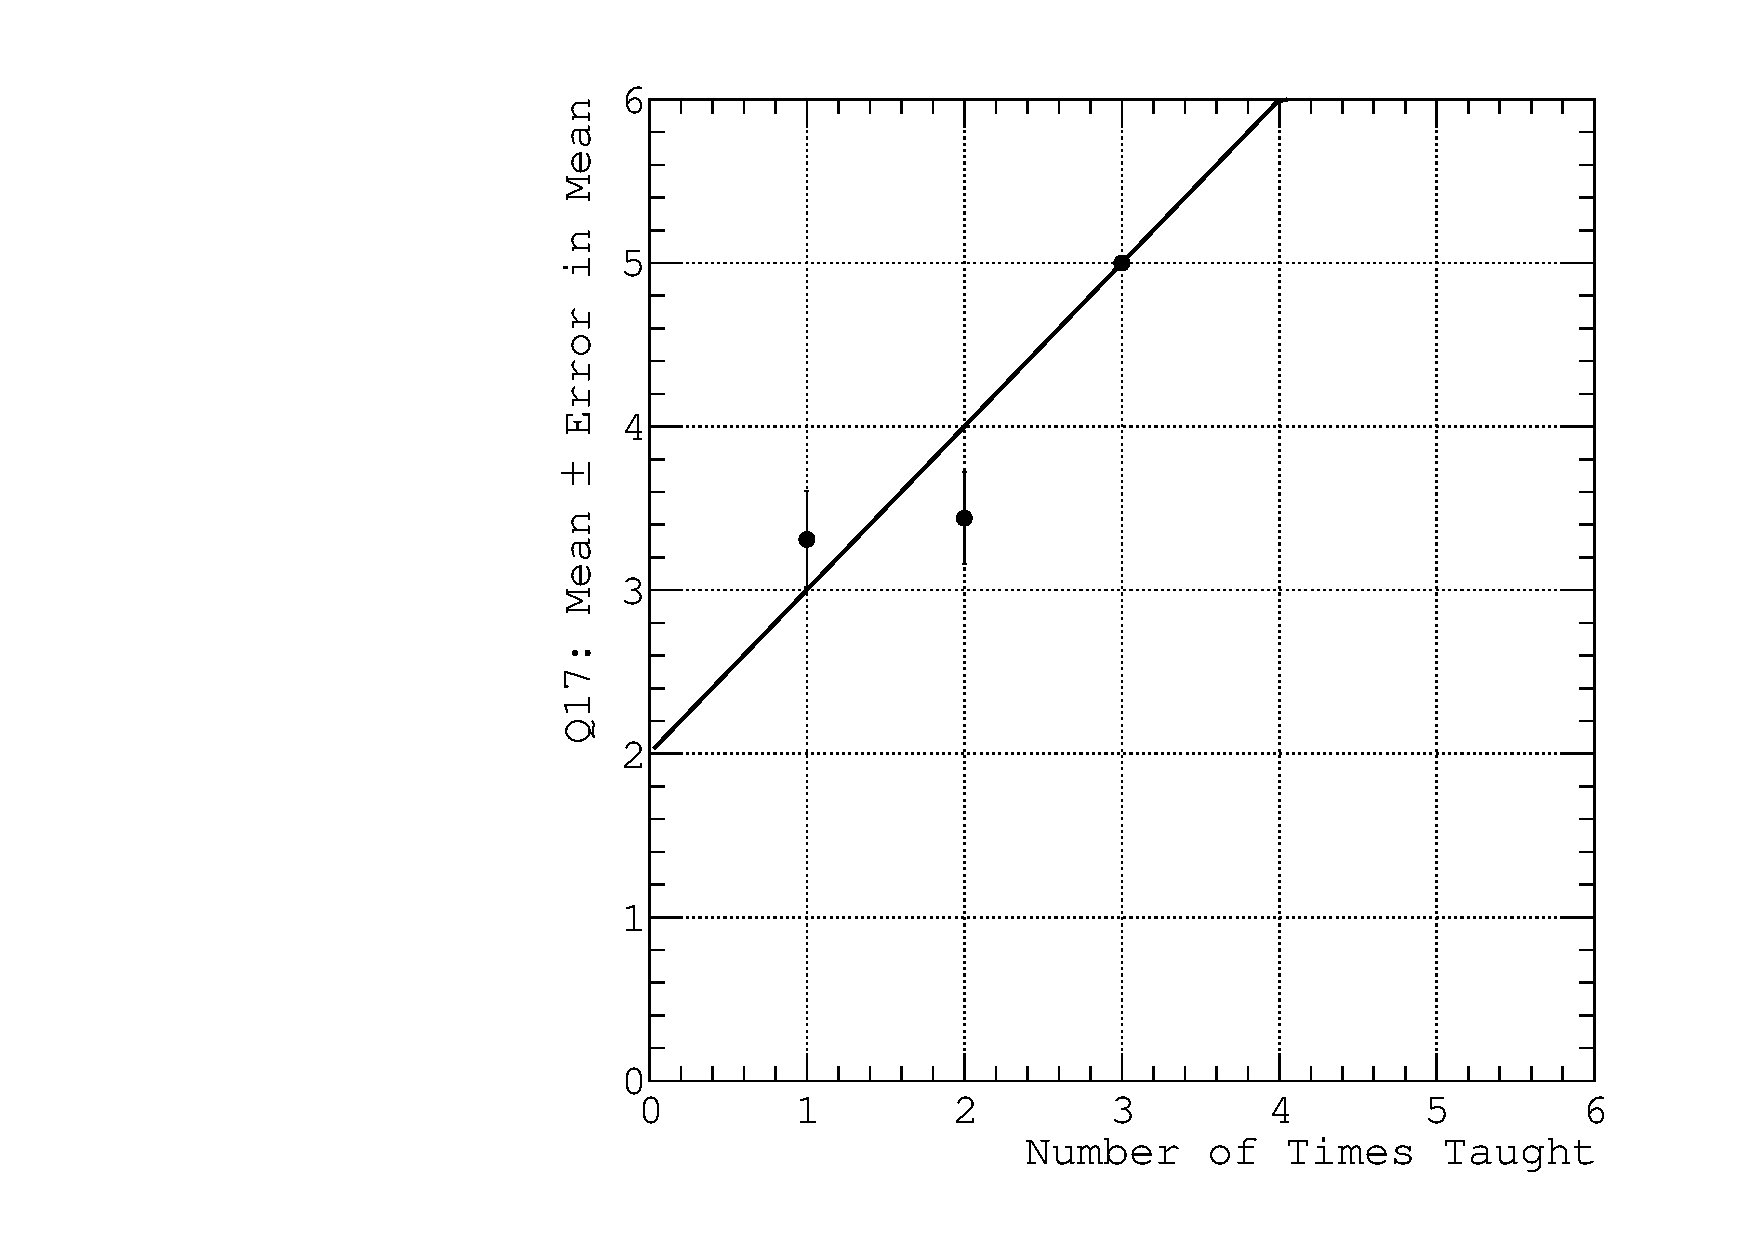
\includegraphics[width=0.4\textwidth]{Q17_calculus_based.pdf}
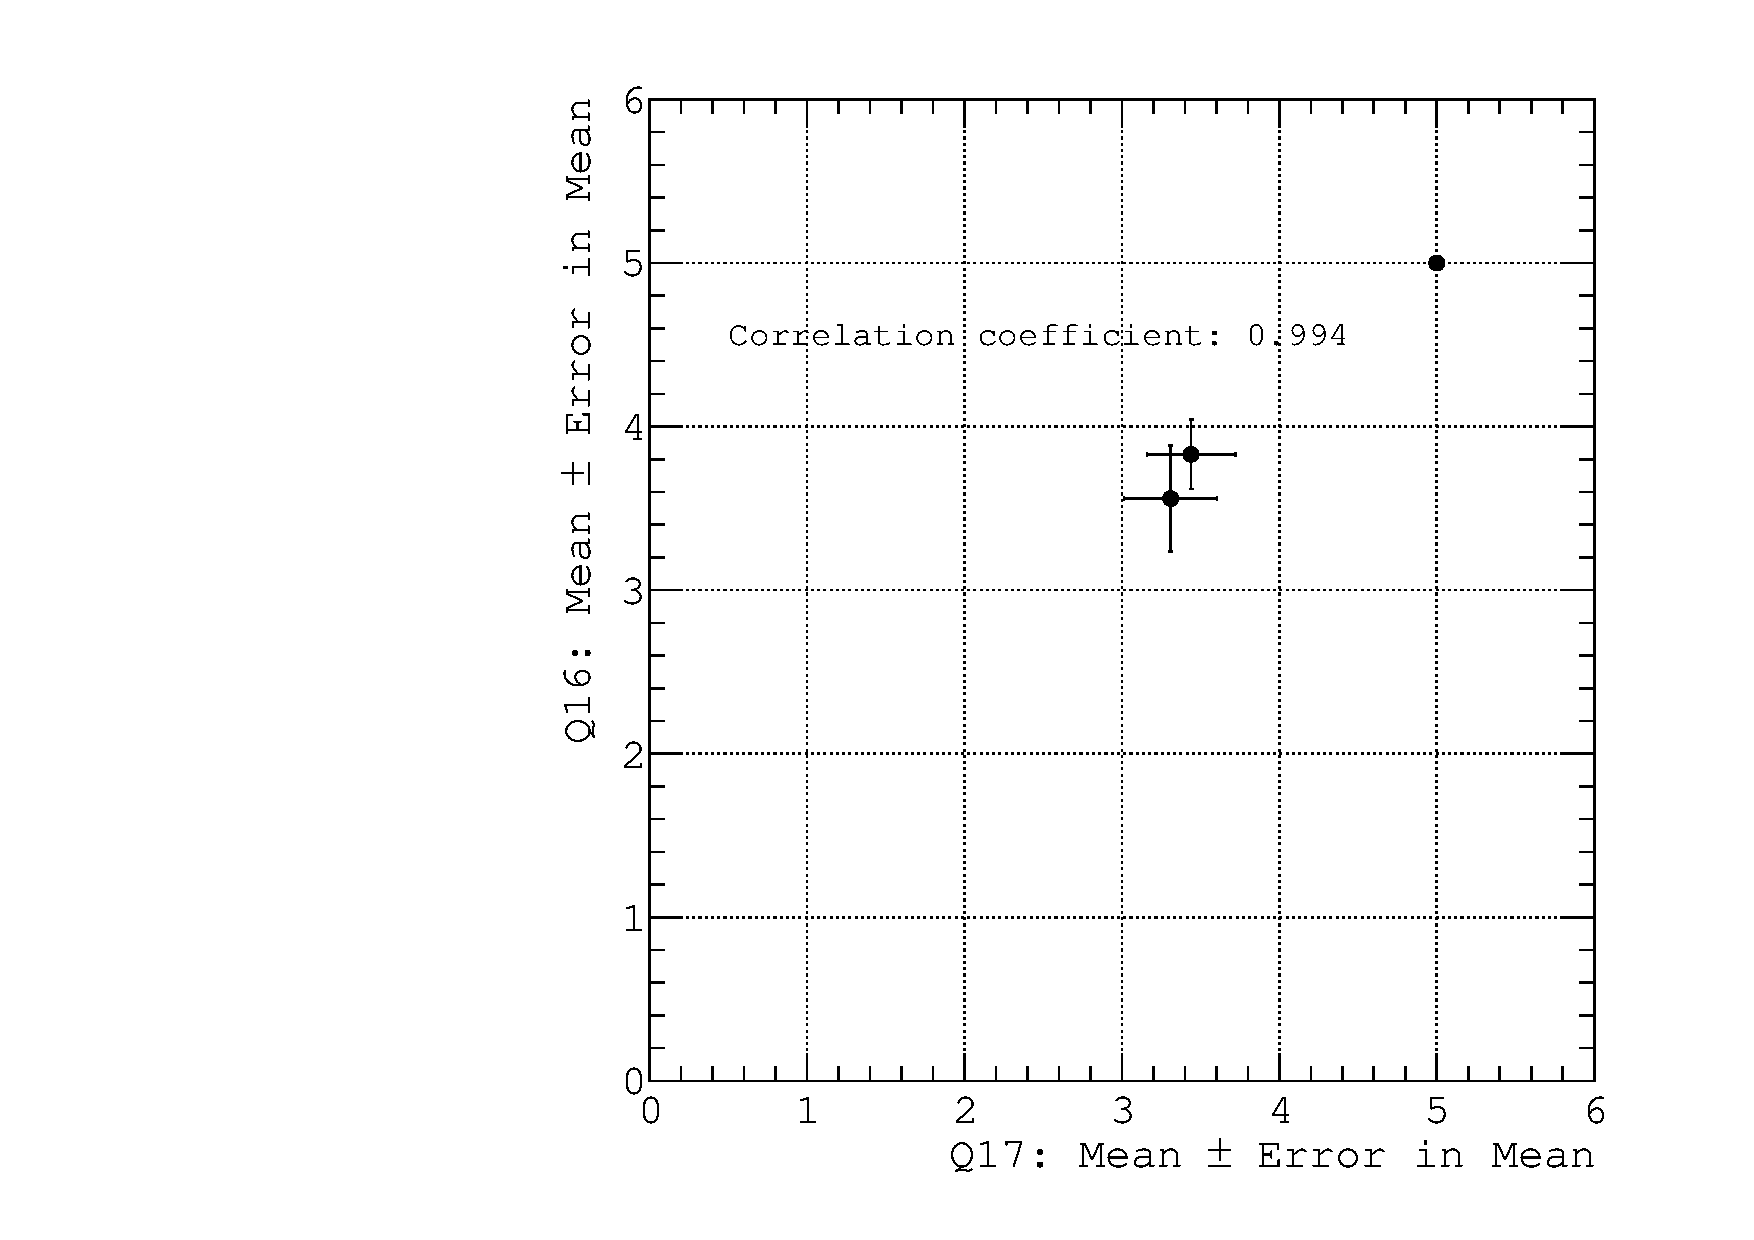
\includegraphics[width=0.4\textwidth]{Q16_Q17_calculus_based.pdf}
\caption{\label{fig:courses:intro_q17_2}  (Left) Student responses (mean values and errors in the mean) to Question 17 in calculus-based physics versus number of times taught. (Right) Student responses to Question 16 in calculus-based physics versus responses to Question 17.  The x and y-axis values of the data points are the mean values, and the errors are the errors in the mean.}
\end{figure}

Similar to algebra-based physics, my department asked me to think about Question 17 mean values\footnote{``The professor used class time effectively and demonstrated preparation for class''.} in the context of calculus-based physics.  Data regarding Question 17 is shown in Fig. \ref{fig:courses:intro_q17_2}.  My department suggested that this measurement is correlated with other key measurements like Question 16.  Figure \ref{fig:courses:intro_q17_2} (right) contains data suggesting this correlation is strong.  The Pearson correlation coefficient is 0.994.  As with algebra-based physics, the JITT modules have been dropped from my calculus-based course style.  What I predict for Fall 2019 is that the data points Questions 16-17 will be between 4 and 5, and that the numbers will remain correlated.  The PHYS150 section upcoming in Fall 2019 will have my advisees in it, but also it is filled to capacity (25).  To further boost responses to Questions 16 and 17, I will introduce pre-lecture material in the form of reading quizzes to ensure the students begin the class on the same page.  This is a technique I have observed in Dr. Lagan's PHYS180 course.  \\ \hspace{0.1cm}

\begin{figure}[hb]
\centering
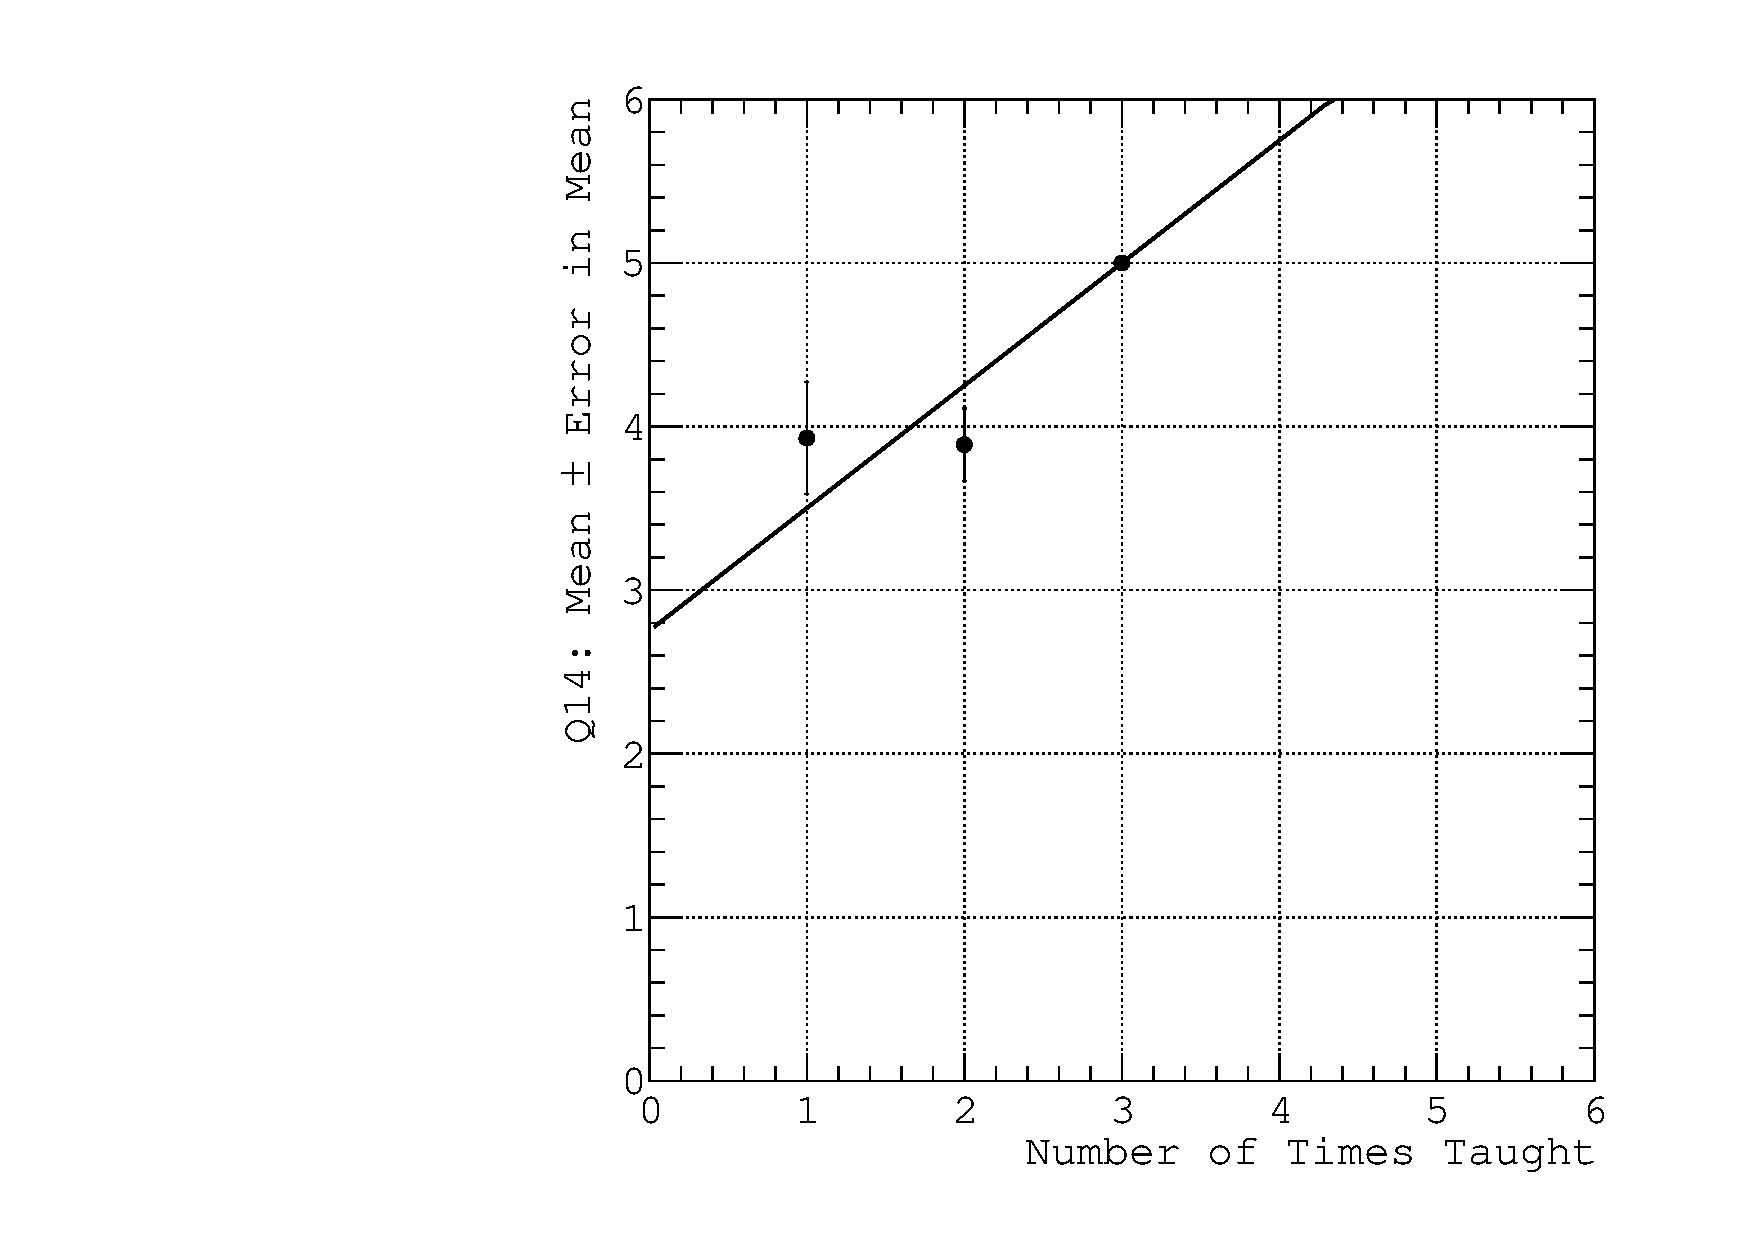
\includegraphics[width=0.4\textwidth]{Q14_calculus_based.pdf}
\caption{\label{fig:courses:intro_q14_2}  Student responses (mean values and errors in the mean) to Question 14 in calculus-based physics versus number of times taught.  The solid black lines are best-fit linear trend lines that minimize the $\chi^2$ value.}
\end{figure}

The second of my three learning focuses for introductory physics courses is to improve the analysis skill of the students.  My strategy of combined traditional and PER based content appears to be working as I improve it over time.  Figure \ref{fig:courses:intro_q14_2} contains student response data to Question 14\footnote{``This course  improved my understanding of the material.''}.  \textbf{The student response data shows that their understanding of the material is improving substantially.}  This was in part due to the aforementioned smaller class size, but also due to the changes I put in place.  During my first two rounds of calculus based physics, the students report an improvement of their understanding of the material consistent with 4.0.  In my most recent calculus-based version, this increased to a 5.0. \\ \hspace{0.1cm}

The third of my introductory learning focuses is \textit{applications to society}, and we served this goal in calculus-based physics in similar ways to algebra-based physics.  The main difference between algebra-based and calculus-based was the sophistication of the student-designed experiments.  Students designed electromagnetic lifting devices (similar to cranes that lift metal objects), and presented elloquently and in quantitative detail (see Supplemental Materials).  Students also chose articles for daily class presentation that they felt had interesting applications to business and engineering.  One student even included an example on how metallurgy is done after learning how to forge metal tools for a project outside of PHYS180. \\ \hspace{0.1cm}

\begin{figure}
\centering
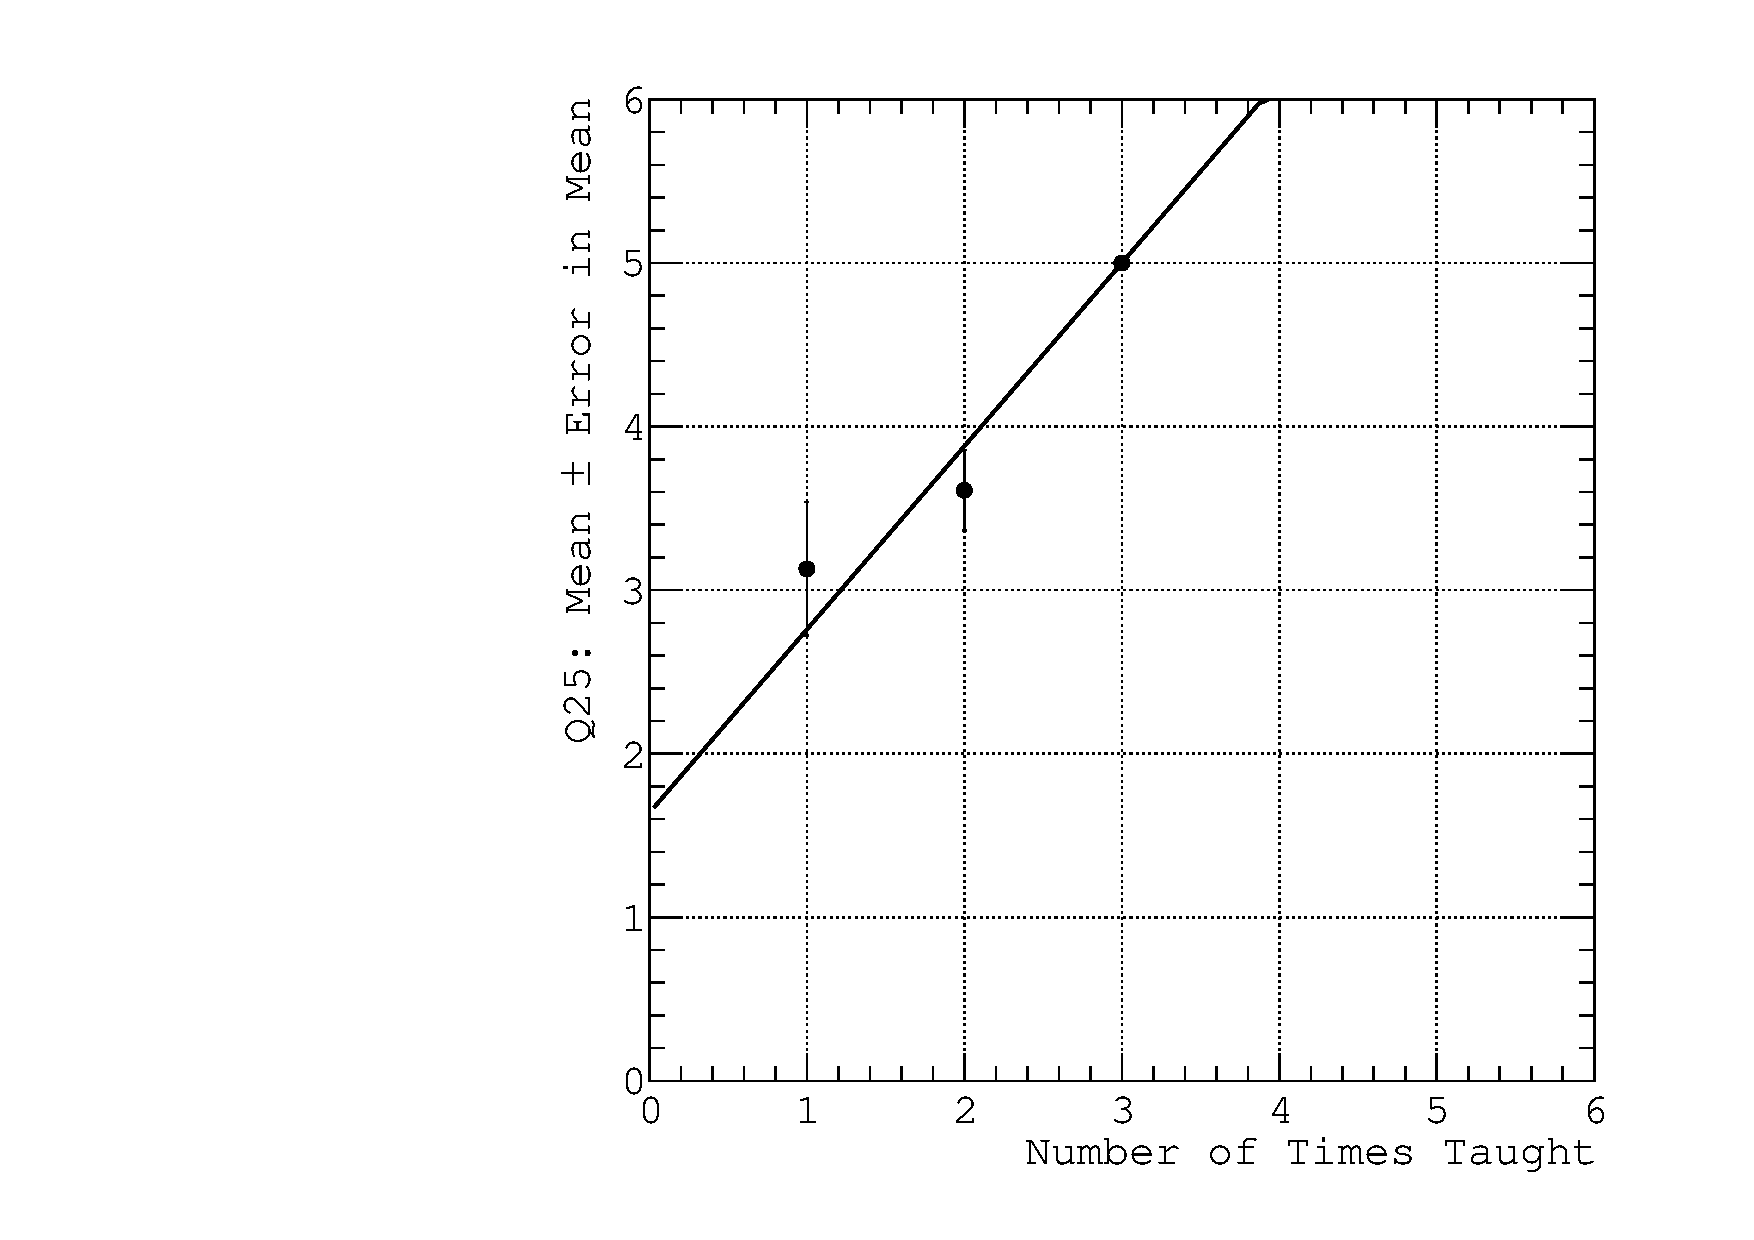
\includegraphics[width=0.4\textwidth]{Q25_calculus_based.pdf}
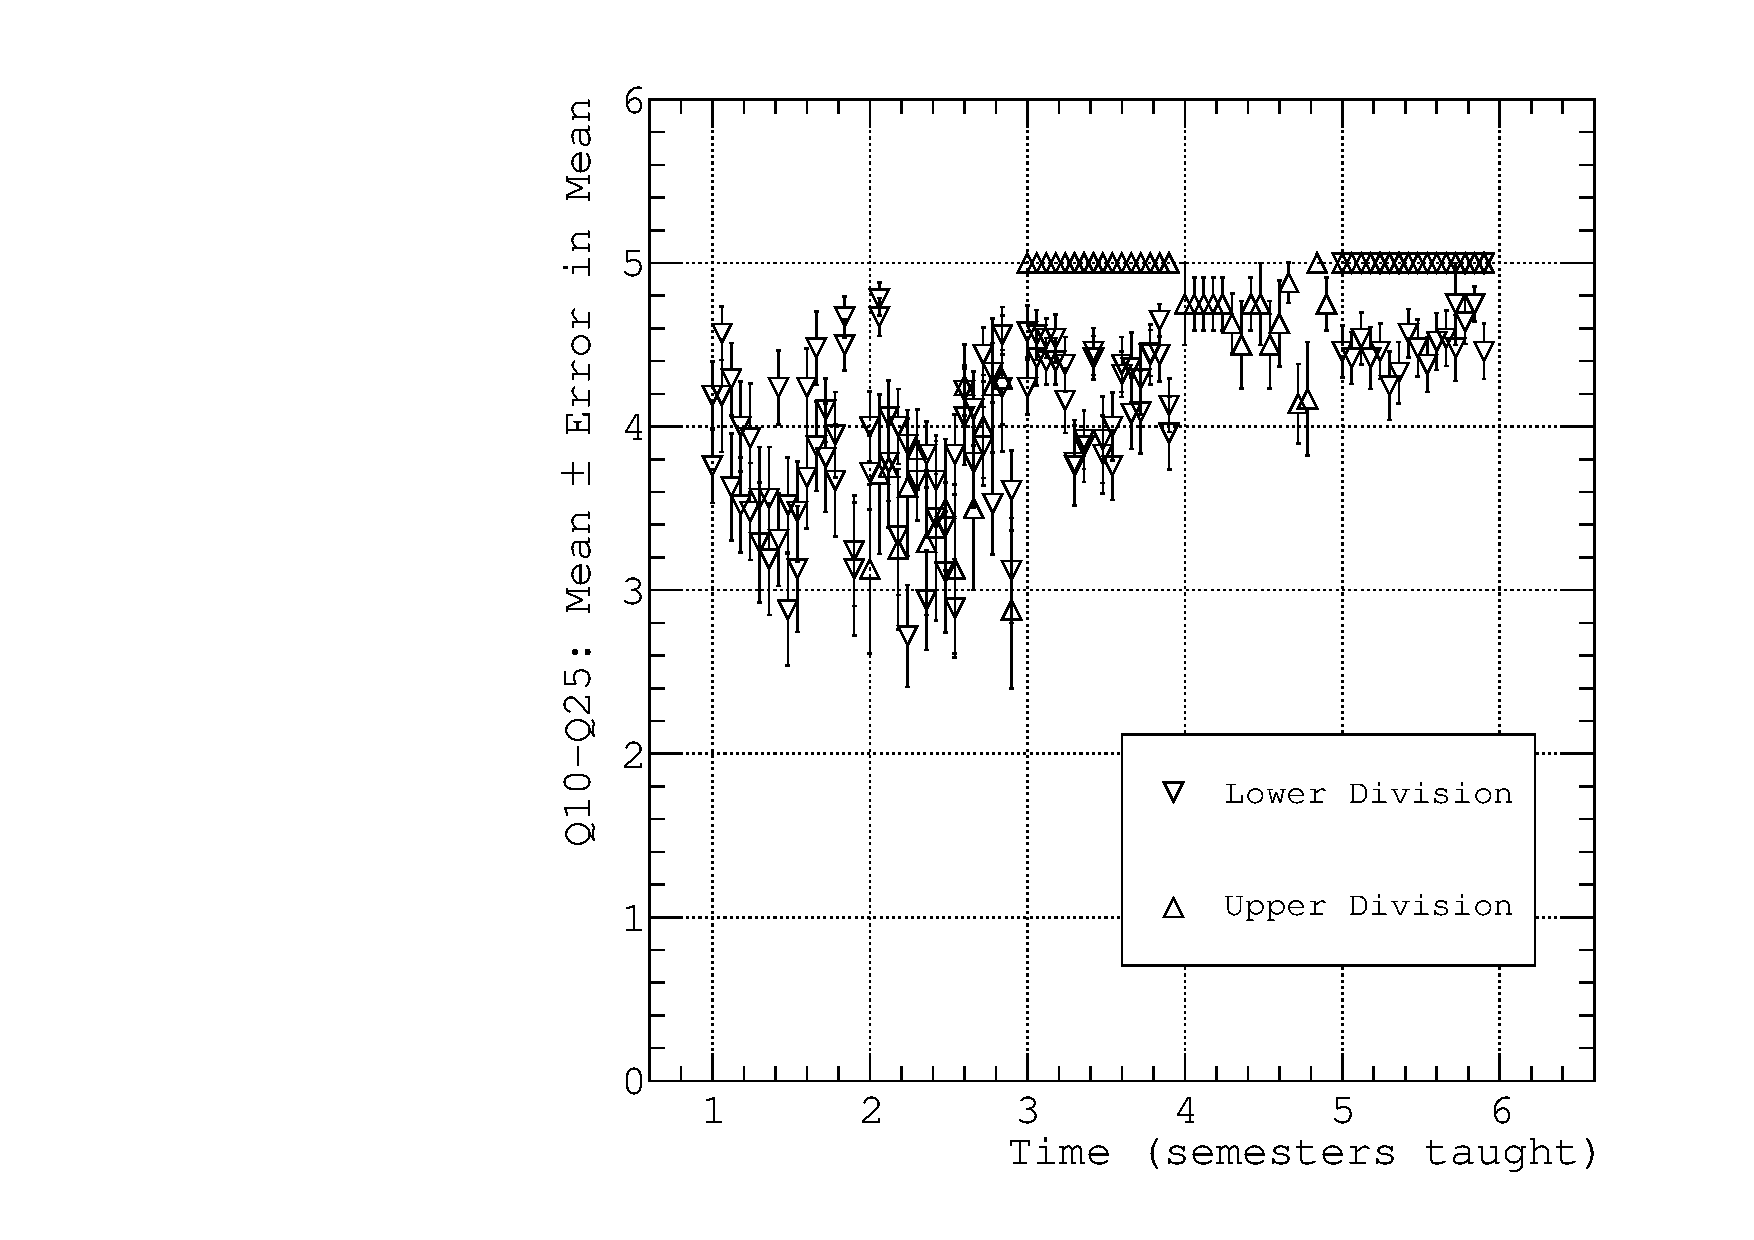
\includegraphics[width=0.4\textwidth]{Q10_Q25_all_courses_vs_time.pdf}
\caption{\label{fig:courses:intro_q25_2}  (Left) Student responses (mean values and errors in the mean) to Question 25 in calculus-based physics versus number of times taught.  The solid black lines are best-fit linear trend lines that minimize the $\chi^2$ value. (Right) Student responses (mean values and errors in the mean) to Questions 10-25 in all courses versus semesters taught at Whittier.}
\end{figure}

Figure \ref{fig:courses:intro_q25_2} (left) contains student response data to Question 25, from calculus-based physics versus time\footnote{``Overall, I would recommend this professor to others.''}.  \textbf{The data show an unmistakable and significant improvement.}  The trend line is driven by the final data point, and as with the other measurements, will likely fall somewhere between 4-5 for Fall 2019 PHYS150 if I continue to refine my approach to the three learning focuses for introductory physics.  To make this point more clearly, I have graphed the mean value responses to \textit{all} questions on the student evaluation form versus semesters taught at Whittier College.  \\ \hspace{0.1cm}

Initially, as I was learning how to serve the diverse student population at Whittier College, the results were mixed.  As time progressed, however, a general trend upwards is observed in all student response data.  There are several courses where the students gave me straight 5.0 scores.  PHYS180 (2019) was one of them, and the other two are two instances of PHYS396 (physics research for credit).  PHYS396 is a course for which we don't receive teaching credit, but is reserved for students who want to do a research project with a physics professor.  The January term of 2019 I denote as the fourth semester, in which I taught COSC390, which was a huge success (see Sec. \ref{sec:oof2}).  Overall, the data show that the students recognize that I care about their learning, and that as I evolve as a professor the methods and modules I execute benefit the students in their minds.  \\ \hspace{0.1cm}

\end{document}